% Chapter 2

\chapter{Modelos de Predicción de los Fen\'omenos Demogr\'aficos: Fertilidad y Mortalidad} % Main chapter title

\hspace{6.5cm}\textit{``All models are wrong, but some are useful''} -- George E. P. Box}

\label{Chapter2} % For referencing the chapter elsewhere, use \ref{Chapter1} 

%----------------------------------------------------------------------------------------

% Define some commands to keep the formatting separated from the content 

\newcommand{\keyword}[1]{\textbf{#1}}
\newcommand{\tabhead}[1]{\textbf{#1}}
\newcommand{\code}[1]{\texttt{#1}}
\newcommand{\file}[1]{\texttt{\bfseries#1}}
\newcommand{\option}[1]{\texttt{\itshape#1}}

%----------------------------------------------------------------------------------------

\section{Introducci\'on}

El incremento en la esperanza de vida, aunque muestra un s\'intoma de progreso social, plantea adem\'as un desaf\'io tanto a los gobiernos como a los planes de pensiones privados y aseguradoras de vida, debido a su impacto en los costes de salud y de las pensiones.\\
Multitud de estudios demogr\'aficos y actuariales han reconocido los problemas causados por una poblaci\'on envejecida, unas bajas tasas de fertilidad y una creciente longevidad, de forma que han centrado la atenci\'on en el desarrollo de t\'ecnicas estad\'isticas para la modelizaci\'on y proyecci\'on de las tasas de fertilidad y mortalidad.\\

Existen claros indicios de que el aumento de la longevidad ser\'a un proceso permanente que se perpetuar\'a de forma indefinida, aunque quiz\'as con periodos de ralentizaci\'on en el futuro. Este aumento en la esperanza de vida en los pa\'ises desarrollados, se produce principalmente pasada la edad de jubilaci\'on, ya que la tasa de mortalidad en esa etapa ya no aumenta de manera exponencial; de hecho:\textit{``esta evoluci\'on de la mortalidad no es f\'acil de explicar mediante factores tradicionales, como son los progresos de la medicina o el aumento de los ingresos y, en la actualidad, constituye un interrogante biol\'ogico, ya que la evoluci\'on de la esperanza de vida entre los humanos es muy superior a la de otros seres m\'as peque\~nos en entornos de laboratorio''} (Siegel y Swanson, 2004, \textcolor{red}{[1]}).\\ 

Este cap\'itulo tiene dos propósitos: por un lado, hacer una revisión de la literatura en torno a estos modelos de predicción y proyección y por otro, describir y analizar los m\'as usados, para, en último término, intentar simular (uno de fertilidad y otro de mortalidad), en la población española y ver cómo se ajustan.\\

Las premisas y desarrollos que a continuaci\'on se exponen a la hora de simular los modelos de fertilidad y mortalidad se asientan sobre la base de los trabajos propuestos por Sevcíková, Alkema y Raftery, (2011)\footnote{El paquete \texttt{\tinysize{\textbf{`bayesTFR'}}} se puede descargar desde \texttt{\tinysize{http://CRAN.R-project.org/package=bayesTRF}}} \textcolor{red}{[2]}, para la \textbf{fertilidad}. Para la \textbf{mortalidad}, nos hemos basado en los modelos no lineales generalizados para definir la familia de modelos de cohortes de edad (GAPC)\footnote{GAPC, Generalized Age-Period-Cohort}, fundamentado, sobre todo, en los trabajos de Lee y Carter, (1992) \textcolor{red}{[3]}, Cairns, Blake y otros, (2011) \textcolor{red}{[4]}, Villegas, Millossovich y Kaishev, (2016) \textcolor{red}{[5]} y Hyndman, Booth y otros, (2014) \textcolor{red}{[6]}, de los cuales y en concreto, los autores de los dos \'ultimos, han desarrollado sendos paquetes\footnote{Los paquetes en cuesti\'on, \texttt{\textbf{`StMoMo'}} y \texttt{\tinysize{\textbf{`demography'}}} est\'an disponibles en \texttt{\tinysize{http://CRAN.R-project.org/package=\\StMoMo}} y  \texttt{\tinysize{http://CRAN.R-project.org/package=demography}}.} bajo el lenguaje de programaci\'on \textbf{\textsf{R}} que permiten implantar y desarrollar la mayor\'ia de modelos estoc\'asticos de mortalidad usados hasta la fecha.\\

En nuestro caso, hemos usado el lenguaje de programaci\'on citado anteriormente con dos prop\'ositos: \textsc{i)} definir y replicar los modelos GAPC de mortalidad estoc\'astica considerados en el estudio de Villegas, Millossovich y Kaishev (2016) y \textsc{ii)} adaptando el modelo a los datos de la poblaci\'on espa\~nola mediante la t\'ecnica de \textit{bootstrapping}\footnote{La t\'ecnica `bootstrapping' (o `bootstrap') es un m\'etodo de remuestreo propuesto por Bradley Efron en 1979. Se utiliza para aproximar la distribuci\'on en el muestreo de un estad\'istico y se usa frecuentemente para aproximar el sesgo o la varianza de un an\'alisis estad\'istico, as\'i como para construir intervalos de confianza o realizar contrastes de hip\'otesis sobre par\'ametros de inter\'es.}, hemos incorporado el par\'ametro basado en la incertidumbre a la hora de estimar y predecir el modelo general de mortalidad de cohortes de edad.

%-----------------------------------------  MODELOS DE FERTILIDAD ---------------------------------------------
\section{Los modelos de proyección de fertilidad: una revisión de la literatura} %Fertilidad: concepto, precisiones y modelos de proyección.

Antes de adentrarnos en la revisión, análisis y aplicación de los modelos de proyección de la fertilidad conviene diferenciar los conceptos de \textit{fecundidad}, \textit{fertilidad} y \textit{natalidad}, los cuales, aún reflejando aspectos diferentes de la demografía, son considerados, algunas veces (sobre todo los dos primeros) como sinónimos; por lo tanto, es importante diferenciar que \textbf{fecundidad} se refiere al número de hijos que se tienen, mientras que \textbf{fertilidad} viene referida a la capacidad biológica de procrear, es decir, a la capacidad de tener hijos. De esta forma, se puede ser fértil y no haber tenido ningún hijo aún, y se puede haber tenido hijos (ser fecundo) y, en cambio, haber perdido la fertilidad. Finalmente, la \textbf{natalidad} \textit{mide la frecuencia de los nacimientos ocurridos en el seno de una población tomada en su conjunto}, (Vinuesa y otros, 1997) \textcolor{red}{[7]}.\\
Normalmente, en demografía la fecundidad se refiere (en palabras de Julio Pérez Díaz)\footnote{Julio Pérez Díaz es científico titular del CSIC e investigador en el Instituto de Economía, Geografía y Demografía. Más datos en: \texttt{\tinysize{https://apuntesdedemografia.com}}} al \textit{número medio de hijos que tiene una generación (normalmente femenina) a lo largo de su vida reproductiva} y aunque vengamos usando, y en lo sucesivo sigamos haciéndolo, la palabra \textit{fertilidad} cuando hablemos de modelos, tasas e índices, realmente deberíamos usar el término \textit{fecundidad}.\\

Además de esto, existen diferentes formas de medir la fertilidad; así, los indicadores más usuales son: la \textit{Tasa General de Fertilidad} (General Fertility Rate, \textsc{gfr}, en sus siglas en inglés), la \textit{Fertilidad Completada} y la \textit{Tasa Total de Fertilidad} (Total Fertility Rate, \textsc{tfr}), siendo éste último el indicador más utilizado. Todos ellos reflejan el comportamiento de la fertilidad de formas `ligeramente' diferentes. Por ejemplo, mientras que la \textit{Tasa General de Fertilidad} muestra la tasa anual en que las mujeres están teniendo hijos actualmente, la \textit{Fertilidad Completada} muestra la cantidad de hijos que tienen en última instancia y la  \textit{Tasa Total de Fertilidad} expresa el número hipotético que probablemente tendrían basado en los patrones de fertilidad actuales.\\
Ninguno es estos indicadores es ``correcto'' o ``equivocado'', o ``mejor' o ``peor'', sin embargo, cada uno muestra una historia diferente cuando la fertilidad toca fondo.\\

El mejor ejemplo que muestra lo anterior lo tenemos en los datos de fertilidad de los Estados Unidos donde se muestran los indicadores mencionados más arriba (ver \textbf{figura 2.1}), en este informe del Centro Nacional de Estadísticas de Salud\footnote{\tinysize{\texttt{http://www.pewresearch.org/fact-tank/2018/01/18/is-u-s-fertility-at-an-all-time-low-it-\\depends/}}}, se utilizó la tasa general de fertilidad para mostrar que la fertilidad de los EEUU en 2016 se encontraba en un mínimo histórico. Por cada 1 000 mujeres en edad fértil, definidas de 15 a 44 años, hubo 62.0 nacimientos.\\

La \textit{Tasa de Fertilidad General} no se ve afectada por el tamaño de la población en general, ni por la proporción de la población que se compone de mujeres en edad fértil. Sin embargo, se ve afectada por cambios en la distribución por edades entre las mujeres en edad fértil; cuanto mayor sea la proporción de mujeres en sus años pico de maternidad, mayor será la tasa general de fertilidad, todo lo demás será igual (y viceversa).\\

Esta tasa que utiliza el gobierno es principalmente el resultado de una disminución en las tasas de natalidad entre las mujeres menores de 30 años, en parte debido a la Gran Recesión de finales de la década de 2000; cuando hay una recesión económica, las personas tienden a posponer tener hijos. Sin embargo, también ha habido un ligero descenso en la proporción de mujeres que están en sus años pico de maternidad (edades 20-34), lo que puede desempeñar un pequeño papel en la disminución.\\

La segunda medida de fertilidad es la \textit{fertilidad completada}, que cuenta el número de hijos que una mujer tiene en su vida. Por lo general, los investigadores recopilan datos sobre la fertilidad de las mujeres de 15 a 44 años de edad porque se consideran años fértiles. Luego miden la `fertilidad completada' como el número de hijos nacidos de mujeres de 40 a 44 años de edad, en el supuesto de que la mayoría de las mujeres a esta edad tienen hijos. De acuerdo con esta medida, desde 1976, el punto más bajo en la fertilidad de los Estados Unidos ocurrió alrededor de 2006, cuando las mujeres cerca del final de sus años fértiles habían tenido un promedio de 1.86 hijos.\\

Debido a que es una medida retrospectiva, la fertilidad completa resume los patrones de maternidad de las últimas décadas, pero no puede proporcionar información directa sobre los comportamientos de fertilidad de las mujeres más jóvenes en la actualidad. Además, debido a que no toma en cuenta la mayor proporción de mujeres que posponen la maternidad, puede subestimar la fertilidad de algunas, como las mujeres altamente educadas, muchas de las cuales tienen hijos más adelante. (Para abordar esto, la Oficina del Censo de los Estados Unidos comenzó recientemente a recopilar datos de fertilidad para mujeres hasta los 50 años).\\

Un tercer indicador, la \textit{tasa de fertilidad total}, es una estimación de la fertilidad de por vida, basada en los patrones de fertilidad actuales. Tocó fondo incluso antes, en el período inflacionario de 1976, cuando se estimó que las mujeres de los Estados Unidos tendrían, en promedio, 1,74 niños en su vida. Este indicador no es un informe real de la fertilidad durante la vida, sino que es una medida hipotética basada en la información de fertilidad de un punto en el tiempo, que luego se proyecta en el futuro para estimar la cantidad de bebés que una mujer típica tendría.\\

\vspace{-0.3cm}
\begin{figure}[!ht]
\centering
%\hspace*{-1.3cm}
\fbox{\includegraphics[scale=0.5]{Cap2/fertus.png}}
\captionsetup{width=0.94\linewidth}
\caption{Indicadores de fertilidad en los Estados Unidos}
\end{figure}

Japón es otro país en el que la tasa de nacimientos se está reduciendo a mínimos históricos, de hecho, en 2018 se produjeron 921 000 nacimientos y 1 370 000 defunciones, hasta el punto de que el país asiático, uno de los más homogéneos y cerrados a la mano de obra exterior, ha aceptado la entrada de 345 000 extranjeros, forzada por el envejecimiento de su población y la baja tasa de natalidad.\\

Con todo, la modelización de las curvas de fertilidad ha sido objeto de interés por parte de los demógrafos desde hace mucho tiempo, de este modo, mediante una amplia variedad de modelos matemáticos, se ha logrado describir que los patrones de fertilidad para edades específicas han tenido una forma común en todas las poblaciones humanas a través de los años. Algunos de estos modelos han resultado verdaderamente efectivos en cuanto al ajuste de las distribuciones de las tasas de fertilidad de la población (Hoem y otros, 1981) \textcolor{red}{[8]}, otros se han mostrado menos eficaces a la hora de estimar esta tarea.\\

Pero, ?`qué propiedades esenciales debe cumplir un modelo de fertilidad? La sostenibilidad de cualquier modelo de este tipo debe ser juzgada en base a las siguientes \textbf{propiedades}:\\

\textbullet\ Debe tener la \textbf{flexibilidad} suficiente para producir la variedad de curvas y niveles necesarios para mostrar los cambios que se produzcan en la distribución.\\

\vspace{-0.3cm}
\textbullet\ Las tasas deben ser \textbf{suavizadas} con respecto a la edad.\\

\vspace{-0.3cm}
\textbullet\ Estas tasas deben ser \textbf{cóncavas} con respecto a la edad; en otras palabras, las tasas deben aumentar monótonamente hasta cierta edad en la que las tasas de fertilidad alcanzan un máximo y luego disminuir monótonamente.\\

\vspace{-0.3cm}
\textbullet\ La \textbf{distribución por edades de la fertilidad no debe ser simétrica}; por lo general, las tasas aumentan desde cero en la menarquia a un máximo entre las edades de 25 y 30 años, aproximadamente 10-15 años después de la menarquia, antes de disminuir durante unos 20-25 años hasta la edad de la menopausia. Por lo tanto, las distribuciones de la tasa de fertilidad tenderán a estar ligeramente inclinadas hacia la derecha.\\

\vspace{-0.3cm}
\textbullet\ Las tasas producidas por un modelo deben ser cero antes de la menarquia y después de la menopausia.\\

\vspace{-0.3cm}
\textbullet\ Deseable, aunque no esencial, que las tasas descritas por el modelo sean analíticamente manejables; es decir, otras propiedades asociadas del programa de fertilidad (la edad media en el parto, la fertilidad acumulada a una edad determinada, por ejemplo) deberían poder ser calculadas con facilidad, ya sea analítica o directamente.\\

Para modelizar la fertilidad se suelen utilizar \textbf{modelos paramétricos} (de forma análoga a los modelos matemáticos de la mortalidad); otro enfoque hace uso de un estándar de fertilidad que puede usarse en un \textbf{modelo relacional} de la misma (al igual que las tablas estándar de vida pueden usarse en modelos relacionales de mortalidad).\\ 

Davis y Blake elaboraron en 1956 el modelo de fecundidad por medio de variables intermedias (Davis y Blake, 1956)\footnote{El sistema análitico de \textit{variables intermedias} consiste en la desagregación del proceso mediante el cual nace una persona, y que gira en torno a tres momentos clave: (1) el coito, (2) la concepción y (3) la gestación y el parto, dando lugar a once variables relacionadas con fecundidad.}\textcolor{red}{[9]}. Dicho sistema fue revisado por Bongaarts, convirtiéndolo en el modelo de \textit{variables próximas} (Bongaarts y Potter, 1983)\footnote{Las \textit{variables próximas} propuestas por Bongaarts parten de tres variables biológicas: (1) el intervalo estéril en el postparto, (2) el intervalo fértil y (3) el tiempo de embarazo completo (asumiéndose una duración constante de 9 meses).}\textcolor{red}{[10]}. De acuerdo con los autores, estas variables son las únicas susceptibles de verse afectadas por factores socioeconómicos y ambientales (según Bongaarts) o culturales (según Davis y Blake). La aplicación del modelo de Bongaarts de fecundidad que hace Josune Aguinaga al caso español resulta interesante desde el punto de vista del contraste entre las Ciencias Naturales y las Sociales, ya que éste modelo, según la autora, es demasiado \textit{`biologicista'} y muy poco `sociológico' y no muestra ninguna relación de causalidad entre ambas realidades, la biológica y la causal (Aguinaga Roustan, 1995) \textcolor{red}{[11]}.\\

Otro tanto sucede cuando, desde un enfoque económico, se intenta averiguar las causas de los cambios en la fecundidad (más allá de factores cuantificables), en este sentido, Del Pino Artacho concluye que de esta óptica, la económica, se antoja insuficiente para esta tarea y que hay otros factores o contextos que infuyen tales como culturales y sociales (Del Pino Artacho, 2005) \textcolor{red}{[12]}.\\
 
Posteriormente, en los modelos desarrollados en los últimos años, los patrones de los datos de fertilidad en los países desarrollados muestran una considerable variación. Esta variación está relacionada con la curva de fertilidad. Ésta, tradicionalmente ha adoptado una forma estándar de campana, ligeramente simétrica aunque más aguda en su parte izquierda alrededor de su pico, en torno a una edad alrededor de los 25 años (Peristera y Kostaki, 2007) \textcolor{red}{[13]}. Según los autores anteriores, ésta comienza con un mínimo colocado al comienzo del intervalo de edad de reproducción y luego aumenta hasta alcanzar un máximo en algún lugar alrededor de los 30 años. Luego vuelve a decrecer para nivelarse cerca de los 50 años.\\
La magnitud de las tasas individuales de fecundidad por edad se ve influenciada por las diferencias en las prácticas matrimoniales y de maternidad; presencia o ausencia de control de la fertilidad y regulaciones sobre la viudez, el divorcio y el nuevo matrimonio, pero el patrón general se ha mantenido sin cambios a través de años y países. Los países muestran desigualdades con respecto a la edad en que las tasas de fertilidad alcanzan un máximo y la velocidad variable con la que se aproxima el máximo desde el principio y luego se pasa para alcanzar el final del período de fecundidad, (Coleman, 1996) \textcolor{red}{[14]}.\\

Países como el Reino Unido, Irlanda y los Estados Unidos muestras patrones de fertilidad heterogéneos, lo cual podría estar asociado en cierta medida al estado civil, así como al nivel educativo y social de las madres. Además, en estos países, esta heterogeneidad en los patrones de fertilidad puede explicarse por las diferencias étnicas en el momento y el número de nacimientos (Sigle-Rushton, 2008) \textcolor{red}{[15]}, (Bray, 2008) \textcolor{red}{[16]}.\\ 

Debido a esta heterogeneidad, los modelos existentes, por lo tanto, no pueden capturar el patrón de fertilidad moderna. Para solventar esto, Chandola y otros, (1999) \textcolor{red}{[17]}, proponen una mezcla de la función de Hadwiger\footnote{La función Hadwiger viene dada según la expresión $h(x)=\frac{\alpha\beta}{\gamma\sqrt{\pi}}\big(\frac{\gamma}{x}\big)^{\frac{3}{2}}exp\big\{-\beta^{2}\big(\frac{\gamma}{x}+\frac{x}{\gamma}-2\big)\big\}$, donde $\alpha$, $\beta$ y $\gamma$ representan los parámetros estimados y $x$ es la edad de la madre al nacimiento del niño.}, (Hadwiger,1940) \textcolor{red}{[18]}, para describir este nuevo patrón de fertilidad que refleje la heterogeneidad del comportamiento de la fecundidad, diferenciando, además la aparición temporal en cada país.\\

Entre los modelos utilizados para representar el patrón de fertilidad específica por edad de poblaciones que no muestran una elevada fertilidad temprana, se ha demostrado que varios de ellos proporcionan ajustes `bastante' precisos a las distribuciones de fertilidad.
Entre ellos destacan, por ejemplo, el modelo de fertilidad paramétrico propuesto por \textit{Coale-Trusell} (Coale y Trussell, 1974; 1978) \textcolor{red}{[19]}, \textcolor{red}{[20]}, el cual sigue siendo ampliamente utilizado hoy día; se trata de un modelo híbrido entre empírico y paramétrico cuya forma básica es $$f(a)=T\cdot G(a)\cdot n(a)\cdot e^{m\cdot v(a)}$$ se trata, por lo tanto, de un modelo de fertilidad con cuatro parámetros \textit{(m, M, a\textsubscript{0} y k)}, más de lo necesario para una representación eficiente. Aunque el modelo tiene la virtud de tener parámetros que tienen algunas interpretaciones del mundo real, estos parámetros no pueden medirse en poblaciones reales, por lo que es difícil ajustar el modelo. Xie (1990)  \textcolor{red}{[21]} y Xie y Pimentel (1992)  \textcolor{red}{[22]}, propusieron extensiones al modelo de Coale-Trussell para hacerlo menos restrictivo y más capaz de capturar la fertilidad en una amplia gama de poblaciones, aunque las modificaciones sugeridas son relativamente menores en términos de su impacto global.\\
También han resultado de gran precisión y son de uso común las distribuciones Beta y Gamma equivalentes a las curvas Tipo I y III de Pearson, respectivamente, propuestas por Hoem y otros (1981) -y mencionada anteriormente-; la misma distribución Hadwiger (también nombrada con anterioridad) y las \textit{splines} cúbicas (Hoem and Rennermalm, 1978) \textcolor{red}{[23]}; (Gilks, 1986) \textcolor{red}{[24]}. Adicionalmente, la \textit{curva de Pearson Tipo I} (Mitra, 1967) \textcolor{red}{[25]}, de \textit{tipo III} (Nurul-Islam and Ali Mallick, 1987) \textcolor{red}{[26]} y el modelo propuesto por Romaniuk (Romaniuk, 1973) \textcolor{red}{[27]} han mostrado un buen ajuste de predicción, ya que todos, de forma directa o indirecta, tienen su origen en el método del ratio \textit{P/F} propuesto por Brass (Brass, 1964) \textcolor{red}{[28]}, que si bien ha sido modificado y reemplazado, en su forma original, por el modelo relacional de Gompertz, la base del método se basa en la observación de que si la fertilidad ha sido constante durante un período prolongado de tiempo, las medidas de fertilidad de la cohorte y el período serán idénticas. Es decir, en condiciones de fertilidad constante, la fertilidad acumulada de una cohorte de mujeres hasta cualquier edad dada será la misma que la fertilidad acumulada hasta esa misma edad en cualquier período dado.\\
Si asumimos que no hay diferencias de mortalidad apreciables por la fertilidad de la madre, de modo que las mujeres sobrevivientes no tengan niveles de maternidad significativamente diferentes a los de las mujeres fallecidas, la fertilidad acumulada de una cohorte de mujeres hasta una edad determinada es la misma que la Paridad Media en esa cohorte (este supuesto no es muy importante, ya que incluso si existen diferencias en la fertilidad de las mujeres vivas y fallecidas, en la mayoría de las poblaciones, la magnitud de la mortalidad femenina en las edades reproductivas es muy pequeña y, por lo tanto, el efecto de la supervivencia diferencial será pequeño).\\
Brass definió \textit{P} como la paridad promedio (fertilidad acumulada de por vida) de una cohorte de mujeres hasta una edad determinada, y \textit{F} se relaciona estrechamente con la fertilidad acumulada (período) hasta esa misma edad. El método de relación \textit{P/F} expresa estas dos cantidades en relación entre sí en forma de una relación para cada grupo de edad.\\

La principal debilidad del método es que en realidad los datos nunca están libres de errores, por lo que el patrón hipotético de desviación de la relación \textit{P/F} de la unidad se confunde con los errores subyacentes en los datos.\\
El segundo tipo de error que se encuentra con frecuencia es que las mujeres tienden a informar cada vez menos de los nacimientos recientes, independientemente de su edad. Los errores de este tipo darán como resultado que el nivel recogido de fertilidad reciente sea algo más bajo de lo previsto, lo que causará que la relación \textit{P/F} se infle.\\

El modelo relacional de Gompertz (Brass, 1974; 1978) \textcolor{red}{[29]}, \textcolor{red}{[30]}, en cambio, se presenta como una mejora m\'as vers\'atil, ya que utiliza los mismos datos de entrada (y hace las mismas suposiciones sobre los errores que afectan los datos de fertilidad) que su precursor. Sin embargo, es importante destacar que el método no requiere el supuesto de que la fertilidad haya sido constante en el pasado. Hemos considerado el modelo relacional Gompertz de fertilidad lo suficientemente importante como para ser explicado más en detalle y aunque si bien por motivos expositivos quizás no procede incluir su desarrollo matemático en este apartado, se ha creído conveniente incluirlo como anexo; de este modo, el lector podrá profundizar un poco más en el funcionamiento del mismo \textit{(ver anexo B)}.\\

Otros tantos autores centran sus análisis en la aplicación y ajuste de los modelos anteriormente descritos a poblaciones específicas y países concretos, por ejemplo, Billari y Kohler, (2002) \textcolor{red}{[31]} usan análisis descriptivos agregados para revisar la relación entre la fertilidad del período bajo y el período bajo más ``bajo'', y la fertilidad de la cohorte y los comportamientos clave relacionados con la fertilidad, como abandonar el hogar de los padres, el matrimonio y la participación de la fuerza laboral femenina, en Europa desde 1975 hasta 1999.\\

DellaPergola, (2007) \textcolor{red}{[32]}, en cambio, enfoca el tema desde la perspectiva de los desarrollos\ en Israel y Palestina discutiendo algunos posibles escenarios futuros para la población emergente, poniendo de manifiesto la variedad de procesos demográficos y sociales que han afectado o pueden afectar al cambio en tamaño y en distribuciones de la población de árabes y judíos en el territorio entre el mar Mediterráneo y el río Jordán.\\

Cai, (2008) \textcolor{red}{[33]}, por su parte, aplica el método `variable-\textit{r}' \footnote{variable-\textit{r} quiere decir `variable rate', esto es, \textit{método de tasa variable.}} de Preston y Coale\footnote{El método de Preston y Coale (Preston, Coale, Trusell y otros, 1980) es el segundo de los métodos que más tarde se conocieron como los \textit{Métodos de Distribución de Muertes}, para estimar la integridad de la notificación de muertes en relación con una estimación de la población en un momento dado, aunque principalmente se utilizan para proyecciones de mortalidad, el enfoque que le dieron Preston y Coale basado en tasas variables, hace que pueda ser utilizado para estimar varias medidas demográficas, como en el caso de Cai, (2008).} para evaluar el nivel de fertilidad en China usando datos del censo así como encuestas de población anual desde 1990 hasta 2000, concluyendo que, con el método propuesto, la fertilidad en el país ha alcanzado un nivel muy por debajo del de reemplazo.\\
Siguiendo con este autor, Yong Cai, junto a Wang Feng (ambos sociólogos), recientemente han publicado un artículo de opinión en el \textit{New York Times}\footnote{\tinysize{\texttt{https://www.nytimes.com/2019/02/26/opinion/china-isnt-having-enough-babies.html}}}, titulado: \textit{`China Isn't Having Enough Babies'}, el cual consideramos interesante comentar. En dicho artículo, se plantean la duda de si el estado puede mantenerse al día con el rápido envejecimiento de una población tan grande. De este modo, muestran que durante el año 2018 hubo 15.23 millones de nuevos nacimientos en el gigante asiático, lo que supone un descenso de más del 11\% con respecto al año 2017, de modo que lo que en un principio habían previsto las autoridades al facilitar y posteriormente abolir, a mediados de la década, la `política de un solo hijo'\footnote{Esta política (en inglés \textit{`one-child policy'}) era parte de un programa de planificación de nacimientos del gobierno chino, introducido en 1979 y diseñado para controlar la población, limitando el número de hijos que podrían tener los padres.} al pronosticar un nuevo baby-boom, más bien se ha convertido en un `baby-bust'\footnote{En contraposición al término `boom' (expansión o explosión), se ha utilizado el término `bust' (depresión o reventón)}.
De acuerdo con los autores, aunque estas cifras no significan que la propia población de China haya comenzado a disminuir, sí significan que la población en general está envejeciendo, y rápido. De hecho, la fertilidad en China comenzó a disminuir, velozmente, a finales de la década de 1960, mucho antes de la entrada, en 1979, oficialmente, de la política de un solo hijo. Al igual que con otros países, las razones incluían una mejor supervivencia de los bebés y niños, y una mayor participación de las mujeres en la fuerza laboral. Y los factores que están reduciendo la fertilidad hoy en día, como la urbanización masiva, la mayor riqueza y más opciones para las mujeres, están teniendo un impacto demasiado fuerte como para no empezar a tenerlos en cuenta, afirman Cai y Feng.\\ 
Paralelamente, aunque argumentan que una baja fertilidad podría tener sus ventajas (menos niños podría conllevar más atención a los actuales en la forma de más inversiones en educación, por ejemplo, lo cual estaría por ver), se une que la esperanza de vida ha aumentado, lo que, significa una carga económica, cada vez mayor, para las personas en edad de trabajar. Todos estos cambios demográficos crean importantes pruebas políticas, tanto ahora, en el presente, como para el futuro. Una es, por ejemplo, cómo mantener el crecimiento a medida que la población sigue envejeciendo y el tamaño relativo de la fuerza laboral sigue disminuyendo. Otra es cómo ofrecer los beneficios económicos y sociales que los chinos ahora esperan del estado. Estas crecientes presiones demográficas debe afrontarlas con reformas sistémicas y, en términos generales, concluyen los autores, \textit{debe proporcionar cuidado infantil adecuado e igual acceso a la educación pública, y garantizar la calidad en la atención médica. Debería posponer la edad de jubilación (actualmente 55 para las mujeres y 60 para los hombres) y nacionalizar los estándares de pensión, en términos más generales, promover la igualdad social, especialmente la igualdad de género, y un equilibrio entre la vida laboral y familiar}.\\

De este modo, Cai expresa la realidad demográfica actual y sus correspondientes desafíos futuros. Tal y como se observa en la \textbf{figura 2.2}, establece que para 2050 habrá 290 millones adicionales de personas con una edad de 55 o más años. El coste de una sociedad envejecida conllevaría, en China, un incremento del 32\% en educación, cuidados de la salud y pensiones y que, de mantenerse los ingresos del gobierno, crearía un déficit de casi el 15\%.\\

\begin{figure}[!ht]
\centering
\hspace*{-0.6cm}
\fbox{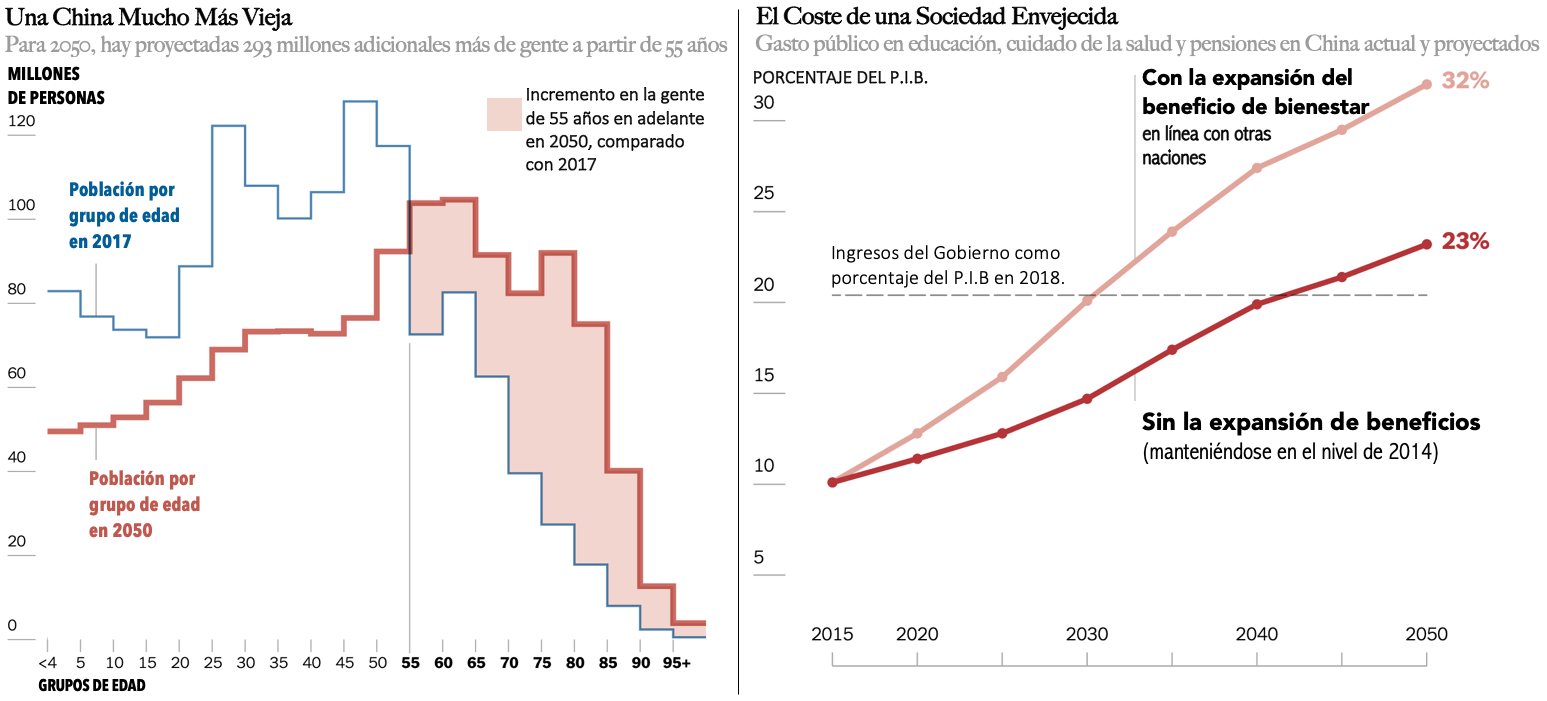
\includegraphics[scale=0.32]{Cap2/china.png}}
%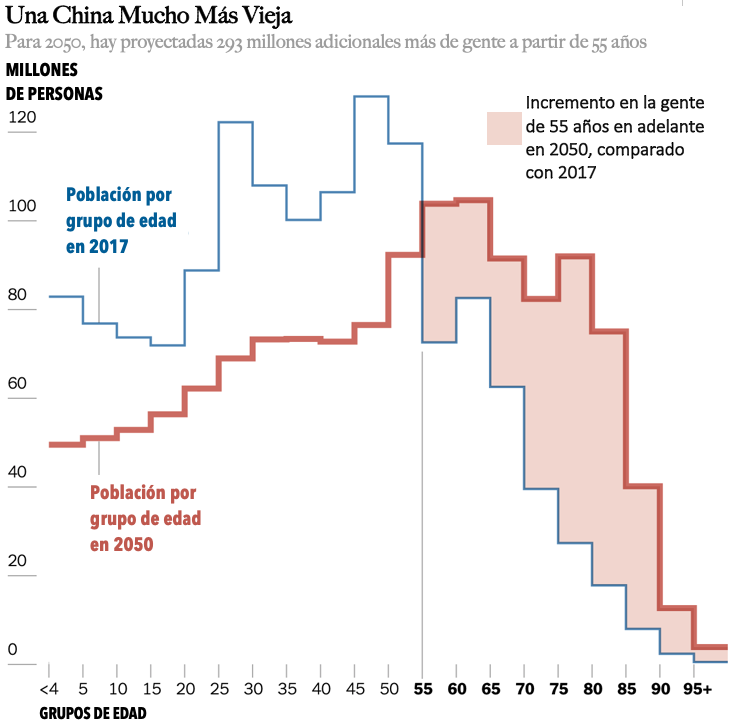
\includegraphics[scale=0.31]{Cap2/oldchina.png}\hspace{0.1cm}\includegraphics[scale=0.33]{Cap2/oldchina2.png}
\captionsetup{width=1.2\linewidth}
\caption[Proyecciones de población y gasto público en China]{\textbf{Izquierda:} Proyecciones de mayores de 55 años. \textbf{Derecha:} Gasto público en educación, salud y pensiones en China}\\
\textit{(Fuente: Adaptación propia a partir de The New York Times y de Yong Cai, Wang Feng y Ke Shen)}
\end{figure}

Continuando con la revisión de la literatura, y siguiendo en el ámbito de los modelos de proyección de la fertilidad, Hyndman y Booth, (2008) \textcolor{red}{[34]}, aplican modelos de datos funcionales y métodos de series de tiempo para pronosticar los componentes del cambio, en la mortalidad, la fertilidad y la migración internacional neta y los usan en el pronóstico de la población de Francia (Booth, Pennec y Hyndman, (2009) \textcolor{red}{[35]}). Dicho pronóstico de la población probabilística se compara con las proyecciones de población oficiales para el país, las cuales están basadas en escenarios deterministas tradicionales.\\

Caltabiano y otros, (2009) \textcolor{red}{[36]}, concentran su atención en Italia; en el estudio de los primeros, el objetivo es describir el proceso de aplazamiento y recuperación del nacimiento en Italia, un país, al igual que España, con niveles persistentes de fertilidad muy bajos, donde encuentran que actualmente se está llevando a cabo una recuperación en las regiones del norte de Italia, signos de recuperación que son, sobre todo, evidentes entre las generaciones más jóvenes y las mujeres con mayor nivel de educación. Siguiendo en Italia, aunque más reciente, De Iaco y Maggio, (2015) \textcolor{red}{[37]}, proponen un modelo dinámico para describir y predecir la evolución de las tasas de fertilidad italianas para una edad específica  a lo largo del tiempo; en concreto, modifican ligeramente la función Gamma para incluir parámetros estocásticos de variación temporal para describir las variaciones sistemáticas y macroscópicas de las tasas de fertilidad específicas por edad a lo largo del tiempo, mientras que se aplica un modelo geoestadístico no paramétrico para describir los residuos correlacionados a nivel microscópico.\\

V\"ahi, (2017) \textcolor{red}{[38]}, por su parte, aporta un nuevo enfoque consistente en mezclar varias distribuciones para predecir el comportamiento reproductivo de la mujer en el futuro. En otras palabras, partiendo de las distribuciones más usadas a la hora de estudiar las curvas de fertilidad, esto es, la distribución gamma, la distribución beta y la función Hadwiger, el autor ha intentado aproximar el método para datos estonios.\\

Para el caso español, interesante es la aportación de Adsera (2004) \textcolor{red}{[39]}, que estudia, en el periodo comprendido entre 1985 y 1999, si la significación de la religión en la fertilidad (tanto en tamaño de la familia como en el intervalo de nacimientos) ha cambiado durante ese lapso de tiempo.\\

Bermúdez y otros, (2012) \textcolor{red}{[40]}, en cambio, proponen un modelo paramétrico para ajustar las curvas de fertilidad basado en una combinación de dos funciones Weibull, dicho modelo desempeña un buen ajuste en países donde la curva de fertilidad muestra un patrón no tradicional y aunque también es adecuado para ajustes de curvas de fertilidad más `clásicos' o dicho de otro modo, para países menos desarrollados donde la fertilidad se viene comportando de la misma forma, el modelo en cuestión depende de tres parámetros y está diseñado principalmente para adaptarse a los patrones de fertilidad en países con una `joroba de edad' temprana\footnote{Por `joroba de edad' se entiende el punto máximo a partir del cual empieza a decrecer la curva.}, concluyendo los autores que si bien no proporciona el mejor ajuste en todos los casos simulados, sí es capaz de mejorar el ajuste que otros modelos, que dependen de más parámetros, proporcionan.\\

\vspace{-0.3cm}
Más reciente y con un enfoque más cuantitativo y técnico, Osés-Arranz y otros (AIReF, 2018) \textcolor{red}{[41]} presentan una metodología para generar proyecciones estocásticas de población que combina el método de cohorte-componente (método de referencia usado en la mayoría de estudios estadísticos en esta materia), con la simulación de Monte Carlo de dos de los principales datos demográficos: tasas de fertilidad (por edad) y probabilidades de supervivencia (por edad y género). La simulación de Monte Carlo se basa en una parametrización de las curvas correspondientes y un modelo multivariante de series de tiempo que se utiliza para simular escenarios futuros. En la parte que viene referida a las proyecciones de fertilidad, los autores concluyen que dicha proyección para España convergerá con la del resto de países europeos también simulados y la cual se sitúa alrededor de 1.8 hijos por mujer.\\

\vspace{-0.3cm}
Para finalizar, no podemos dejar de echar un vistazo (ver \textbf{figura 2.3}) a la situación actual europea en cuanto a lo anteriormente descrito se refiere, es decir, en el siguiente gráfico se muestran, por un lado, la media de edad al tener el primer hijo en los países de la UE y por otro, la tasa de fecundidad, en nacimientos por mujeres. Vemos que España, con 30.9 años de media es, junto a Italia, Grecia e Irlanda (y Suiza) de los países en los que las mujeres tienen su primer hijo más tarde, todas se encuentran por encima de los 30 años. A la vez, estos mismos países (exceptuando a Irlanda) se encuentran a la cola en cuanto a tasa de fecundidad, en torno a 1.30 hijos por mujer. ¿Por qué coinciden geográficamente tantos países europeos con baja fecundidad? Parece ser que el retraso en dejar el hogar familiar es clave. En palabras de Albert Esteve\footnote{Director del Centro de Estudios Demográficos de Barcelona}: \textit{``en los países del sur la emancipación es tardía, y los jóvenes dependen del apoyo que les puedan dar sus familias. Además, cuando se emancipan no tienen hijos inmediatamente, ya que al empezar una relación de pareja hay un tiempo de prueba hasta saber si es la ideal para ser el padre o madre de los hijos''}.

\vspace{-0.1cm}
\begin{figure}[!ht]
\centering
%\hspace*{-1.3cm}
\fbox{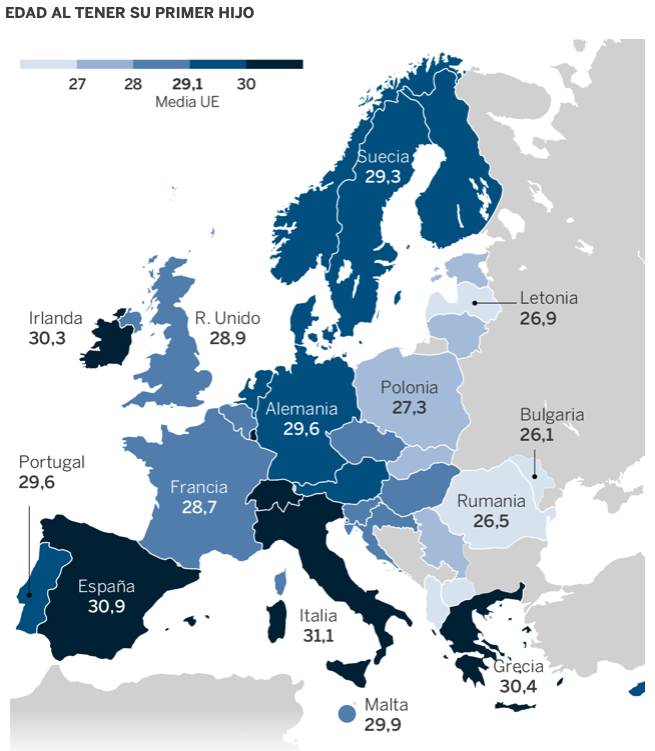
\includegraphics[scale=0.405]{Cap2/edadprimer.png}\hspace{0.2cm}\includegraphics[scale=0.46]{Cap2/tasafec.png}}
\caption{Media de edad al tener el primer hijo y tasa de fecundidad en la Unión Europea}\\
\textit{(Fuente: Eurostat)}
\end{figure}


\subsection{Ajuste y proyección en la poblaci\'on espa\~nola del modelo 'bayesTFR'}

Tras analizar los modelos de proyección de la fertilidad más usados, el siguiente paso es simular el ajuste y la proyección en la población española. Esta parte es importante en el conjunto de la obra, pues sienta una de las bases de futuras investigaciones en el área de predicción y simulación de modelos demográficos.\\
Tal y como apuntamos al principio, para nuestra simulación nos hemos basado en los trabajos de Sevcíkovà y otros, (2011) y Alkema, Raftery y otros, (2011) \textcolor{red}{[42]}, los cuales proponen un modelo de proyección bayesiano\footnote{La estadística bayesiana es una rama de la estadística basada en el teorema de Bayes. La inferencia bayesiana no usa valores-\textit{p} y generalmente no prueba hipótesis. Requiere que se especifique, formalmente, una distribución de probabilidad que recoja el conocimiento previo sobre, por ejemplo, un efecto de tratamiento. El estado del conocimiento previo puede especificarse como ``sin conocimiento previo'' mediante el uso de una distribución, aunque puede llevar a estimaciones sin mucho sentido. Una vez especificada la distribución anterior, los datos se utilizan para modificar el estado de conocimiento previo para obtener el estado de conocimiento posterior al experimento. Las probabilidades finales calculadas en el marco bayesiano son probabilidades con diversos efectos de tratamiento. El precio de poder calcular probabilidades subjetivas sobre el proceso de generación de datos es la necesidad de especificar una distribución previa para fijar los cálculos de partida.} para estimar la tasa total de fertilidad (TFR), tasa que recordemos, es uno de los componentes clave en las proyecciones de población y, que como se ha definido previamente (en concreto en el \textit{\textbf{anexo B}}, cuando se hizo referencia al modelo relacional Gompertz de fertilidad de Brass), es el \textit{número medio de hijos que una mujer tendría si sobreviviera hasta el final de la edad reproductiva experimentando en cada edad las tasas de fertilidad específicas de la edad de ese período}.\\
Las Naciones Unidas produce proyecciones de la \textit{Tasa Total de Fertilidad} \textsc{(tfr)} para 196 países; estas tasas son revisadas cada dos años y publicadas en el \textit{World Population Prospects}, (2017) \textcolor{red}{[43]}; en nuestro caso hemos simulado este mismo modelo usado por las Naciones Unidas con el paquete en \textsf{\textbf{R}} creado para ello y `testado' y usado por varios analistas de dicha organización. Dicho paquete está disponible desde la plataforma Comprehensive \textsf{\textbf{R}} Archive Network (\textsc{cran}) en \texttt{\small{http://CRAN.R-project.org/package=bayesTFR}}.

\subsubsection{Metodología técnica del modelo de proyección de fertilidad}

El modelo de proyección bayesiano propuesto por Alkema y otros \textcolor{black}{[42]} y sobre el cual se basa el paquete \textbf{`bayesTFR'} disponible en \textsf{\textbf{R}}, usa estimaciones de 5 años de la tasa total de fertilidad desde 1950-1955 hasta 2005-2010 y está basado en la observación de que la evolución de la TFR (Tasa Total de Fertilidad) incluye tres amplias fases, referidas como, \textit{Fase I}: una fase de alta fertilidad pre-transicional; \textit{Fase II}: la transición a la fertilidad en la cual la TFR decrece desde niveles de fertilidad altos hacia o por debajo del nivel de fertilidad de reemplazo y la \textit{Fase III}, una fase posterior a la transición de baja fertilidad, que incluye la recuperación de la fertilidad por debajo del reemplazo hacia la fertilidad de reemplazo y las oscilaciones alrededor de la fertilidad a ese mismo nivel. El período de observación para cada país se divide en estas diferentes fases en función de las definiciones deterministas de sus períodos de inicio y finalización, y luego se modela por separado. Por tanto, se define $\tau_{c}$ como el comienzo de la \textit{Fase II} para el país $c$, la cual es dada por
\[
  \tau_{c}=\begin{cases}
             \text{max}\{t:(M_{c}-L_{c,t})< 0.5\}, \hspace{0.5cm} \text{si}\ L_{c,t}>5.5;\\
              < 1950-1955, \hspace{2.5cm} \text{en otro caso},
            \end{cases}
\]
donde $M_{c}$ es el resultado de la TFR máxima observada en el país $c$, y $L_{c,t}$ indica el máximo local. El periodo de comienzo de la \textit{Fase III}, indicado por $\lambda_{c}$ para el país $c$ se observa dentro del período de observación si se han observado dos aumentos posteriores por debajo de una TFR de 2. Para esos países, $$\lambda_{c}=\text{min}\{t:f_{c,t}>f_{c,t-1},f_{c,t+1}>f_{c,t}\ \text{y}\ f_{c,p}<2\hspace*{0.3cm} \text{para}\ p=t-1,t,t+1\}$$ donde $f_{c,t}$ es la TFR en el país $c$ y en el periodo $t$. Para el resto de países, $\lambda_{c}>2005-2010$. El método propuesto, según los autores, no modela la \textit{Fase I}, se trata tal cual es, no obstante, si algún país se encuentra en esta fase, se asume que en la \textit{Fase II} en el siguiente periodo, por lo que esta primera fase no es relevante para las proyecciones.\\

\textbullet\hspace{0.2cm} \textsc{el modelo para la fase ii: la transición a la fertilidad}\\

La fase de transición a la fertilidad es modelizada por un proceso aleatorio con deriva, el cual viene especificado por
\begin{equation}
f_{c,t+1}=f_{c,t}-d_{c,t}+\varepsilon_{c,t},\text{para}\ \tau_{c}\leq t<\lambda_{c},
\end{equation}
donde $f_{c,t}$ es la TFR en el periodo $t$ a cinco años en el país $c$, $d_{c,t}$ es el término decremental que modela el declive sistemático durante la transición a la fertilidad, $\varepsilon_{c,t}$ es una distorsión aleatoria que modela la desviación del deterioro sistemático, $\tau_{c}$ es el periodo de comienzo del declive en la fertilidad y $\lambda_{c}$ es el periodo de comienzo de la \textit{Fase III} post-transicional definida anteriormente.\\
Las distribuciones de las distorsiones aleatorias en cada periodo están dadas por
\[
  \varepsilon_{c,t}\sim\begin{cases}
             N(m_{t},s_{t}^{2}) \hspace{1cm} \text{para}\ t=\tau_{c},\\
             N(0, \sigma(f_{c,t})^{2}) \hspace{0.4cm} \text{en otro caso},
            \end{cases}
\]

donde $m_{\tau}$ es la media y $s_{\tau}$ es la desviación típica de la distorsión en el periodo de comienzo. La cantidad $\sigma(f_{c,t})$ es la desviación típica de las distorsiones durante los periodos posteriores, dada por la expresión 
$$\sigma(f_{c,t})=c_{1975}(t)\big(\sigma_{0}+(f_{c,t}-S)(-aI_{[S,\infty)}(f_{c,t})+bI_{[0,S)}(f_{c,t}))\big),$$
donde $\sigma_{0}$ es la desviación típica máxima de las distorsiones, alcanzada al nivel $S$ de la TFR, y $a$ y $b$ son multiplicadores de la desviación típica para modelar la disminución lineal para resultados mayores y más pequeños de la TFR. La constante $c_{1975}(t)$ es añadida para modelar la varianza de error más alta de las distorsiones antes de 1975, y viene dada por
\[
  c_{1975}(t)=\begin{cases}
             c_{1975},\hspace{0.2cm} t\in [1950-1955, 1970-1975];\\
            1,\hspace{0.8cm} t\in [1975-1980, \infty).
            \end{cases}
\]
El decremento $d_{c,t}$ en (1.1) es modelado como una función del nivel de la TFR como sigue:
\begin{equation}
d_{c,t}=d(\boldsymbol{\theta}_{c},\lambda_{c},\tau_{c},f_{c,t}) =
\begin{cases} 
      g(\boldsymbol{\theta}_{c},f_{c,t}) & \text{para}\ f_{c,t}> 1; \\
      0 & \text{en otro caso}
   \end{cases}
\end{equation}
donde $g(\cdot,\cdot)$ es una función de disminución paramétrica. Esta función especifica una disminución a cinco años (decrecimiento) como función del nivel normal de la TFR y el vector $\boldsymbol{\theta}$. La función de disminución es la suma de dos funciones logísticas, es decir, una función logística doble o bi-logística (según detalla las Naciones Unidas, Dpto. de Asuntos Sociales y Económicos, División de Población, 2017). La función logística doble con el parámetro vector específico para cada país $\boldsymbol{\theta}=(\bigtriangleup_{c1},\bigtriangleup_{c2},\bigtriangleup_{c3},\bigtriangleup_{c4},d_{c})$ es dada por
$$\frac{-d_{c}}{1+\text{exp}\Big(-\frac{2\text{ln}(p_{1})}{\bigtriangleup_{c1}}(f_{c,t}-\sum_{i}\bigtriangleup_{ci}+0.5\bigtriangleup_{c1})\Big)}+\frac{d_{c}}{1+\text{exp}\Big(-\frac{2\text{ln}(p_{2})}{\bigtriangleup_{c3}}(f_{c,t}-\bigtriangleup_{c4}+0.5\bigtriangleup_{c3})\Big)},$$
donde $d_{c}$ es el máximo ritmo posible de la disminución, $p_{1}=p_{2}=9$ son constantes y los $\bigtriangleup_{ci}'s$ describen los rangos de la TFR en los cuales el ritmo de la disminución de la fertilidad cambia, donde $U_{c}=\sum_{i=1}^{4}\bigtriangleup_{ci}$ es el nivel de comienzo de la disminución de la fertilidad (ver \textbf{figura 2.4}).\\
Los parámetros de la función de disminución son estimados para cada país. Para países en los cuales el periodo de comienzo $\tau_{c}$ de la transición a la fertilidad está dentro del periodo de observación, el nivel de comienzo $U_{c}$ se fija en la TFR en ese periodo, $U_{c}=f_{c,\tau_{c}}$. Para los países en los que la transición comenzó antes del período de observación, el nivel de inicio se agrega como un parámetro al modelo, con distribución previa $$U_{c}\sim(\text{min}\{5.5,\operatorname*{max}_t f_{c,t}\},8.8).$$

\vspace{-0.3cm}
\begin{figure}[!ht]
\centering
%\hspace*{-1.3cm}
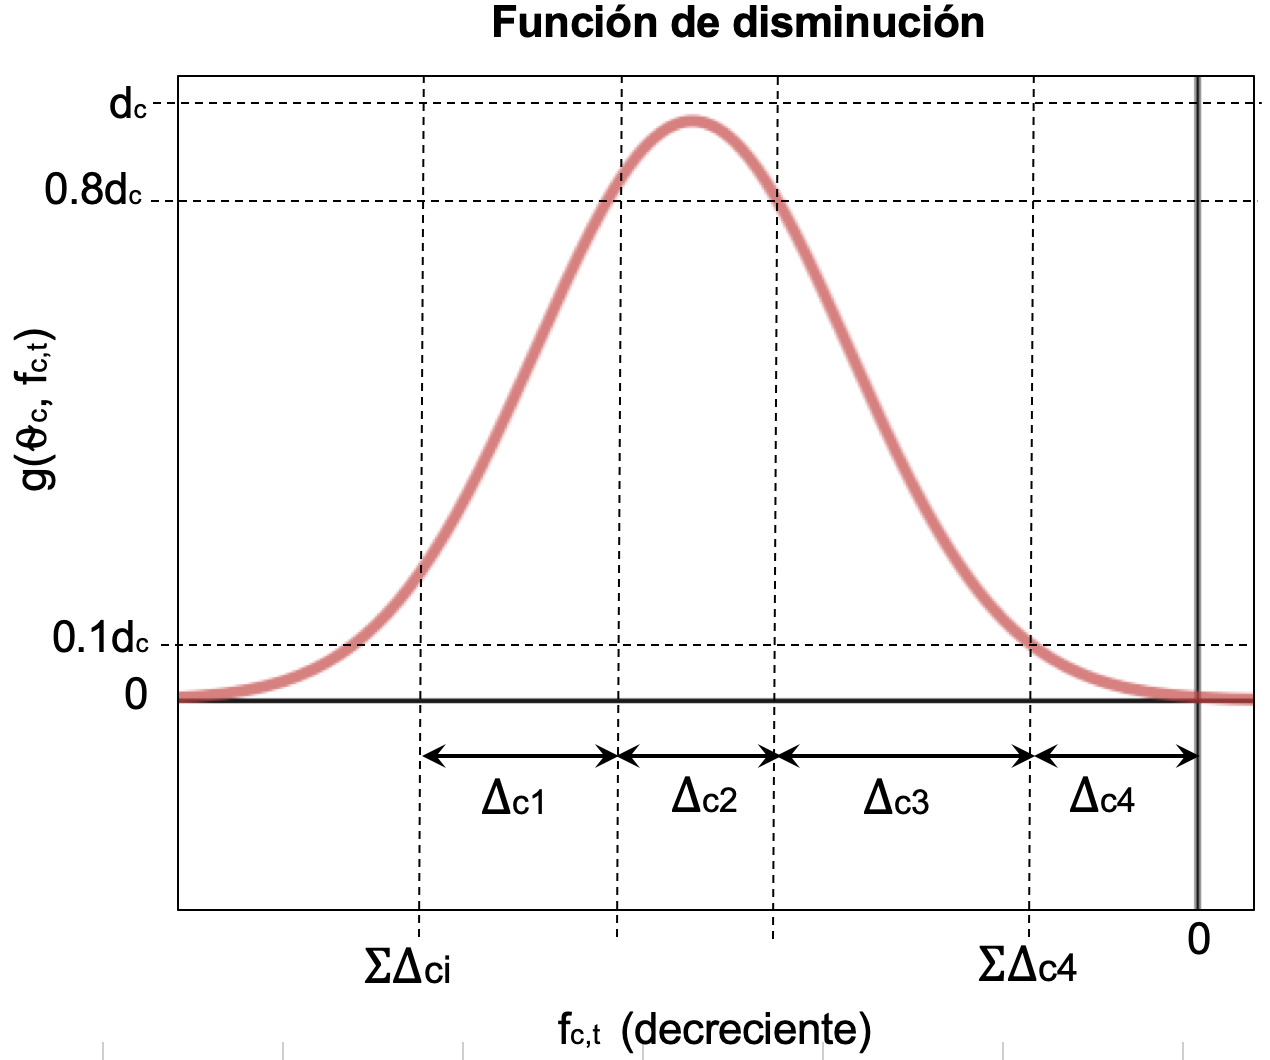
\includegraphics[scale=0.4]{Cap2/decline.png}
\captionsetup{width=0.94\linewidth}
\caption[Disminuciones de cinco años dadas por la función logística doble]{Disminuciones de cinco años, como indica la función de doble declive logístico $g(\boldsymbol{\theta},f_{c,t})$ trazada contra la TFR. El eje horizontal TFR está orientado de forma negativa (es decir, disminuye de izquierda a derecha)}
\end{figure}
Dado el nivel de comienzo $U_{c}$, los cinco parámetros  que determinan el ritmo de la disminución de la fertilidad y el tiempo que toma la transición en el país $c$ son: $\bigtriangleup_{c4}, \{\bigtriangleup_{ci}/(U_{c}-\bigtriangleup_{c4}):i=1,2,3\}$, y, $d_{c}$.\\
Para estimar los parámetros en cada país, los autores usan un modelo jerárquico Bayesiano (Lindley y Smith, 1972 \textcolor{red}{[44]}; Gelman y otros, 2004 \textcolor{red}{[45]}) y que viene dado por:

\begin{align*}
\vspace{-2cm}
d_{c}^{*} & = \text{log}\bigg(\frac{d_{c}-0.25}{2.5-d_{c}}\bigg), \\ 
d_{c}^{*} & \sim N(\chi, \psi^{2}),\\
\bigtriangleup^{*}_{c4} & = \text{log}\bigg(\frac{\bigtriangleup_{c4}-1}{2.5-\bigtriangleup_{c4}}\bigg), \\
\bigtriangleup^{*}_{c4} & \sim N(\bigtriangleup_{4}, \delta^{2}_{4}),\\
p_{ci} & = \frac{\bigtriangleup_{ci}}{U_{c}-\bigtriangleup_{c4}}\text{para}\ i=1,2,3,\\
p_{ci} & = \frac{\text{exp}(\gamma_{ci})}{\sum_{j=1}^{3}\text{exp}(\gamma_{cj})},\\
\gamma_{ci} & \sim N(\alpha_{i}, \delta_{i}^{2}),
\end{align*}
con media y varianza de parámetros $\{\chi, \psi^{2}, \bigtriangleup_{4}, \delta_{4}, \boldsymbol{\alpha, \delta}\}$.\\

En la fase de modelización post-transición el cambio en la TFR se modeliza, según los autores, por un modelo de serie temporal autorregresivo de primer orden, es decir, AR(1) con una media fijada, aproximadamente, al nivel de fertilidad de reemplazamiento, $\mu=2.1$:
\begin{equation}
f_{c,t+1}\sim N(\mu+\rho(f_{c,t}-\mu),s^{2})\ \text{para}\ t \leq \lambda_{c},
\end{equation}
donde $\rho$ es el parámetro autorregresivo con $|\rho|<1$ y $s$ es la desviación típica de los errores aleatorios. Ambos parámetros se estiman por máxima verosimilitud.\\

Finalmente, las proyecciones de la TFR durante la transición a la fertilidad para los países que se encuentran en la \textit{Fase II} se basan en el modelo de esta fase, como se ha visto anteriormente, utilizando la muestra de la distribución posterior de los parámetros del modelo.\\
Como observación final, los autores puntualizan que: \textit{``la mediana (y no la media) se utiliza como la mejor `proyección' debido a su clara interpretación y robustez al comportamiento de la cola de las distribuciones posteriores: independientemente de la forma de la distribución posterior, la mitad de las trayectorias de la TFR están arriba, y la mitad de las trayectorias están por debajo de la mediana''.}

\subsubsection{Uso, ajuste y proyecciones obtenidas del modelo `bayesTFR'}

Como mencionamos anteriormente, este modelo ha sido implantado en un paquete en \textsf{\textbf{R}}, llamado \textbf{`bayesTFR'} y que ha sido el que hemos intentado ajustar para proyectar la TFR en el caso de España; estas proyecciones probabilísticas incluyen límites de incertidumbre y que en el caso de países menos desarrollados, con menos datos disponibles o cuyas entradas más recientes de datos observados no existen, son más destacables.\\

Desde un punto de vista computacional, para obtener dichas proyecciones, se han seguido tres pasos en el siguiente orden:\\

\noindent 1. Ajuste del modelo de proyección TFR, para lo cual:\\
\indent (a) Se ha calculado el periodo de comienzo de la \textit{Fase II} y el periodo de comienzo de la \textit{Fase III} para cada país ($\tau_{c}$ y $\lambda_{c}$). Esta fase, en nuestro caso, es común a todo el proceso, aunque luego, posteriormente, nos hayamos centrado en España.\\
\indent (b) Se ha obtenido una muestra posterior de los parámetros del modelo de Fase II utilizando el algoritmo MCMC\footnote{Markov Chain Monte Carlo}.\\

\noindent 2. Se han generado futuras trayectorias de la TFR (este paso incluye la estimación de los parámetros del modelo AR(1) en la \textit{Fase III} usando el método de estimación de máxima verosimilitud).\\

\noindent 3. Se han analizado los resultados utilizando un conjunto de funciones que resumen, trazan, diagnostican y exportan los resultados de los dos pasos anteriores.\\

En nuestro caso, detallamos a continuación la secuencia lógica de ejecución para el paso 1, es decir, el ajuste del modelo de proyección TFR, si bien el resto del código se muestra en el \textit{(anexo \textbf{f})}, para que pueda ser comprobado.\\ 

{
\setlength{\fboxsep}{0.75pt}%
\noindent\setlength{\fboxrule}{0pt}%
\fbox{%
{\colorbox{gray!20}{\parbox{1\linewidth}{%
\small{\texttt{>\ simulation.dir <- file.path(getwd(), "fertsimul")\\
>\ m1 <- run.tfr.mcmc(nr.chains = 5, iter = 10000, + output.dir = simulation.dir)\\
>\ m1 <- run.tfr.mcmc(nr.chains=5, iter=10000, output.dir=simulation.dir, seed=1)\\
>\ m2 <- continue.tfr.mcmc(iter=1000, output.dir=simulation.dir)
}}}}}}}\\

La primera línea del código crea un directorio donde se almacenarán todas las simulaciones que se hagan, a partir de ahí, mediante la función \texttt{run.tfr.mcmc} se produce el ajuste de la proyección TFR. Dependiendo del tamaño de la muestra MCMC, los pasos 1(b) y 2 son bastante largos en cuanto a su ejecución se refiere, en nuestro caso, la expresión \texttt{nr.chains} determina el número de cadenas MCMC a simular y dado que el objetivo es hacer funcionar el modelo con una base realista, hemos simulado cinco cadenas de 10 000 iteraciones cada una, adicionalmente, simulamos otras 1 000 iteraciones, haciendo un total de 11 000 iteraciones, lo cual nos llevó alrededor de seis horas. Todos estos resultados se almacenaron en el directorio creado al efecto.\\

Una vez creadas las simulaciones, procedimos a crear las trayectorias con la siguiente función:\\

{
\setlength{\fboxsep}{0.75pt}%
\noindent\setlength{\fboxrule}{0pt}%
\fbox{%
{\colorbox{gray!20}{\parbox{1\linewidth}{%
\small{\texttt{>\ pred1 <- tfr.predict(sim.dir = simulation.dir, end.year = 2100, burnin = 2000, + nr.traj = 3000, verbose = TRUE)
}}}}}}}\\

Donde se eliminarán 2 000 simulaciones al principio de cada cadena y se usarán 3 000 valores de parámetros de las restantes 5 cadenas de 9 000 simulaciones cada una, es decir, 45 000 iteraciones para generar las trayectorias. A modo de resumen mediante el comando \texttt{summary}:\\

{
\setlength{\fboxsep}{0.75pt}%
\noindent\setlength{\fboxrule}{0pt}%
\fbox{%
{\colorbox{gray!20}{\parbox{1\linewidth}{%
\small{\texttt{>\ summary(m3, meta.only = TRUE)}\\

{\color{blue}{
\texttt{MCMC parameters estimated for 196 countries.\\
Hyperparameters estimated using 196 countries.}\\

\texttt{WPP: 2008\\
Input data: TFR for period 1950 - 2010  .}\\

\texttt{Number of chains = 5\\
Iterations = 1 : 55000\\
Thinning interval = 1\\
Chains sample sizes: 11000, 11000, 11000, 11000, 11000}
}}}}}}}}\\

Donde vemos que los datos simulados con MCMC y los hiperparámetros $\{\chi, \psi^{2}, \bigtriangleup_{4}, \alpha_{i}, \delta_{i}, \delta_{4}}\}$ son para 196 países.\\

Centrándonos ya en España, con los siguientes comandos obtendremos toda la información relativa y necesaria para nuestro país:\\

{
\setlength{\fboxsep}{0.75pt}%
\noindent\setlength{\fboxrule}{0pt}%
\fbox{%
{\colorbox{gray!20}{\parbox{1\linewidth}{%
\small{\texttt{>\ summary(m3, country = "Spain", par.names = NULL, thin = 10, burnin = 2000)}
}}}}}}}}\\

\noindent la cual, a modo de extracto se muestra en la siguiente salida obtenida de la simulación:\\

{
\setlength{\fboxsep}{0.75pt}%
\noindent\setlength{\fboxrule}{0pt}%
\fbox{%
{\colorbox{gray!20}{\parbox{1\linewidth}{%
\color{blue}{
\small{\texttt{Country: Spain}\\ 

\texttt{Iterations = 2010:11000}\\
\texttt{Thinning interval = 10}\\ 
\texttt{Number of chains = 5}\\ 
\texttt{Sample size per chain = 600}\\ 

\texttt{1. Empirical mean and standard deviation for each variable, plus standard error of the mean:}}

%\begin{table}[h!]
\ttfamily{
\begin{tabular}{ccccc}
  & Mean   &   SD  & Naive SE 	   &   Time-series SE\\
delta_1   & 0.87805 	& 0.222604  & 0.0040642   &   0.0242830\\ 
delta_2  & 0.93463 & 0.290494 & 0.0053037   &   0.0444689\\ 
delta_3  &  0.85959 &	0.205225  & 0.0037469  &    0.0243039\\ 
Triangle4  & 0.49771 &	0.312075 & 0.0056977  &    0.0266451\\
delta4  & 1.18525 &	0.657369 	& 0.0120019   &   0.1198672\\
U\_c724      &      	7.23997 	&0.942422 &	0.0172062   &   0.0172611\\
d\_c724       &     	0.15115  &	0.057671 & 	0.0010529  &    0.0015251\\
Triangle\_c4\_c724  &	1.77613 &	0.343262 	 & 0.0062671   &   0.0105829\\
gammat\_1\_c724    & 	0.06726 &	0.069615 	& 0.0012710   &   0.0018478\\
... & & & &
\end{tabular}}\\

2. Quantiles for each variable:\\

\ttfamily{
\begin{tabular}{cccccc}
   &   	2.5\%  &    25\%  &     50\%  &     75\%  &   97.5\% \\
delta_1   & 0.50418  &  0.71747  & 0.86230  & 	1.01957  & 1.34928\\
delta_2     &   0.47444  & 	0.73158 &  	0.90539  & 	1.08324  	& 1.65377\\
delta_3    &     0.48672  & 	0.71673  & 	0.85140  & 	0.98991  & 	1.29804\\
Triangle4  &    -0.09077  & 	0.31455  & 	0.51002  & 	0.69595  & 	1.04759\\
delta4     &   0.54755  & 	0.85690  & 	1.06003  & 	1.29358  & 	3.32724\\
... & & & & &
\end{tabular}}
}
}}}}}}\\

\noindent y mediante la función \texttt{pred2}, podremos obtener los estadísticos para para las trayectorias proyectadas:\\

{
\setlength{\fboxsep}{0.75pt}%
\noindent\setlength{\fboxrule}{0pt}%
\fbox{%
{\colorbox{gray!20}{\parbox{1\linewidth}{%
\small{\texttt{>\ summary(pred2, country = "Spain")}\\
}}}}}}}}
\vspace{-0.5cm}

{
\setlength{\fboxsep}{0.75pt}%
\noindent\setlength{\fboxrule}{0pt}%
\fbox{%
{\colorbox{gray!20}{\parbox{1\linewidth}{%
\color{blue}{
\small{\texttt{Country: Spain}\\ 

\texttt{Projections: 17 ( 2018 - 2098)}\\
\texttt{Trajectories: 3000}\\ 
\texttt{Phase II burnin: 2000}\\ 
\texttt{Phase II thin: 10}\\ 
\texttt{Parameters of AR(1):}\\
\texttt{mu rho sigma}\\
\texttt{2.1 0.886 0.102}\\

\texttt{Projected TFR:}\\

%\begin{table}[h!]
\ttfamily{
\begin{tabular}{cccccccccccc}
  & Mean  &  SD &  2.5\% &  5\%  & 10\%  & 25\%  & 50\%  & 75\%  & 90\%  & 95\% & 97.5\%\\
2013 & 1.33 & 0.000 &  1.33 & 1.33 & 1.33 & 1.33 &	1.33  & 1.33 & 1.33 & 1.33 & 1.33\\
2018 & 1.41 & 0.102 & 1.21 & 1.24 &  1.28 & 1.34 & 1.41 & 1.48  & 1.54 & 1.58 &  1.61\\
2023 & 1.49 & 0.135 & 1.21 & 1.26 & 1.31 & 1.40 & 1.49 & 1.58 &  1.66 & 1.71 & 1.75\\
2028 & 1.56 & 0.157 & 1.25 & 1.30 &  1.36 & 1.45 & 	1.56 & 1.67 & 1.77 & 1.81 &  1.86\\
2033  & 1.62 & 	0.171 & 1.29 & 	1.33 & 1.40  & 1.51 & 1.62 & 1.74 & 1.84 & 1.91 & 1.96\\
2038  & 1.68 & 	0.183 & 1.32 &	1.38 & 1.44 & 1.56 &	1.68 & 1.80 & 1.92 & 1.98 & 2.04\\
... & & & & & & & & & &
\end{tabular}}
}
}}}}}}\\

\newpage
La representación gráfica (\textbf{figura 2.5}) arroja las siguientes simulaciones:

\begin{figure}[!ht]
\centering
\hspace*{-1cm}
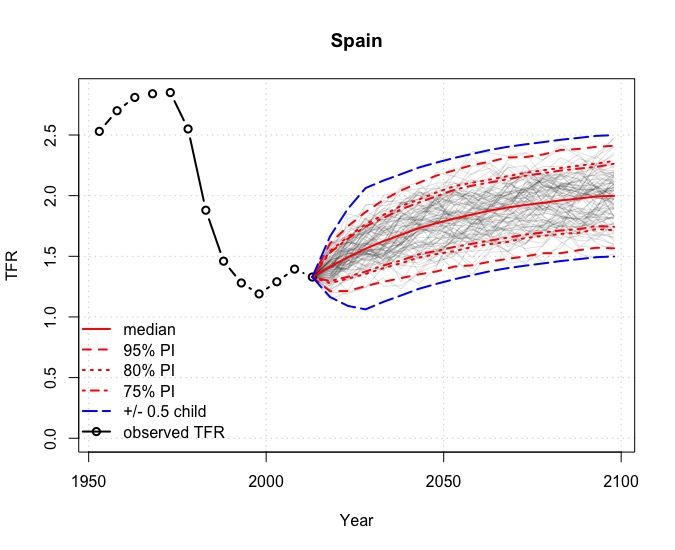
\includegraphics[scale=0.4]{Cap2/bayesTFR01.jpeg}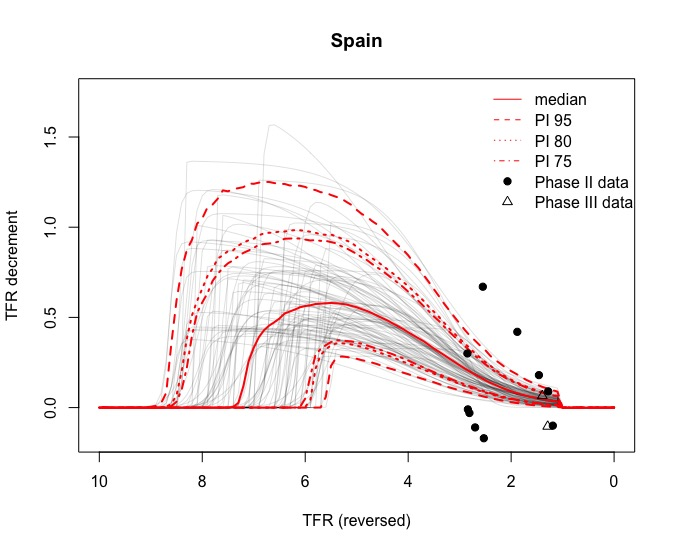
\includegraphics[scale=0.4]{Cap2/bayesTFR02.jpeg}
\captionsetup{width=1.05\linewidth}
\vspace{-0.7cm}
\caption[Proyecciones probabilísticas de la fertilidad total usando estimaciones de fertilidad WPP de 2017]{\textbf{Izquierda:} proyecciones probabilísticas de la fertilidad total usando las estimaciones de fertilidad WPP de 2017. Proyecciones de la fertilidad total: Mediana, 80\%, intervalos de predicción del 95\% y variante de la fertilidad alta/baja. \textbf{Derecha:} Proyecciones probabilísticas de fertilidad total usando las estimaciones de fertilidad (WPP 2017) Curvas de disminución (basadas en la función logística doble) del modelo jerárquico bayesiano, Mediana, 80\% e intervalos de predicción del 95\%.}\\
\textit{(Fuente: Elaboración propia en \textbf{R} con el modelo \textbf{bayesTFR} a partir de Naciones Unidas - WPP)}
\end{figure}

En la gráfica de la izquierda, observamos las proyecciones del modelo jerárquico bayesiano de fertilidad total realizadas con las estimaciones de la \textit{`World Population Prospects. Revision 2017'}. Hay que tener en cuenta que solo se muestra una pequeña selección de las trayectorias probabilísticas de fertilidad total (líneas grises) para la ilustración. La proyección mediana es la línea roja sólida en negrita, y los intervalos de proyección del 80\% y 95\% se muestran como líneas rojas discontinuas y de puntos, respectivamente. Las variantes de fertilidad alta-baja corresponden a +/- 0.5 niños alrededor de la trayectoria media mostrada como líneas discontinuas azules. El nivel de reemplazo de hijos por mujer estaría en el nivel 2.1, aunque no se muestra en la gráfica.\\

En la gráfica de la derecha, se muestran de las curvas de disminución también del modelo jerárquico bayesiano (BHM) de la fertilidad total que se han realizado con las estimaciones de fertilidad de la \textit{`World Population Prospects. Revision 2017'}. Al igual que en el modelo anterior, se ha de tener en cuenta que solo se muestra una pequeña selección de las trayectorias probabilísticas logísticas dobles (líneas grises) para la ilustración. Los decrementos de cinco años observados por el nivel de fertilidad total se muestran con puntos negros si se refieren a los períodos de la transición de fertilidad definidos como Fase II (es decir, de fertilidad alta a baja). La proyección mediana es la línea roja sólida en negrita, y los intervalos de proyección del 80\% y 95\% se muestran como líneas rojas discontinuas y de puntos, respectivamente. Los datos de la Fase I se refieren al período anterior al inicio de la transición de fertilidad (si ocurrió desde 1950). Los datos de la Fase III se refieren al período posterior a la transición de baja fertilidad no modelizado utilizando el modelo logístico doble, sino mediante un modelo de serie temporal autorregresivo de primer orden, AR(1).\\

La \textbf{conclusión principal} a la que llegamos tras la simulación del modelo para España es que el ajuste es bastante preciso ya que el dato de partida sitúa la tasa de fecundidad alrededor de 1.3 nacimientos por mujer, dato similar al que proporcionaba el \textit{Eurostat} en la \textit{figura \textit{2.2}}. Además de esto, lo verdaderamente interesante son las proyecciones que hace el modelo y que se puede comprobar se van aproximando a la tasa de 1.8 nacimientos por mujer, tasa que concuerda con las proyecciones que realiza la AIReF (Osés-Arranz y otros, 2018 [41]) y que comentamos anteriormente cuando hablamos de los modelos de proyección para el caso español.\\

La simulación de las iteraciones para los hiperparámetros $\{\chi, \psi^{2}, \bigtriangleup_{4}, \alpha_{i}, \delta_{i}, \delta_{4}}\}$ pueden ser igualmente analizadas y exploradas gráficamente usando dos funciones del paquete: una para visualizar los parámetros independientes del país, y la otra para visualizar los parámetros del país específico, lo cual, en \textsf{\textbf{R}}, viene dado por el comando\\

\vspace{-0.3cm}
{
\setlength{\fboxsep}{0.75pt}%
\noindent\setlength{\fboxrule}{0pt}%
\fbox{%
{\colorbox{gray!20}{\parbox{1\linewidth}{%
\small{\texttt{>\ tfr.partraces.plot(mcmc.list = m3, par.names = "Triangle4", nr.points = 100)}
}}}}}}}}\\

\vspace{-0.3cm}
\noindent para la gráfica $\bigtriangleup_{4}$, (izquierda) que contiene un rastro por cada cadena MCMC (en nuestro ejemplo 5 rastros).

\begin{figure}[!ht]
\centering
\hspace*{-1cm}
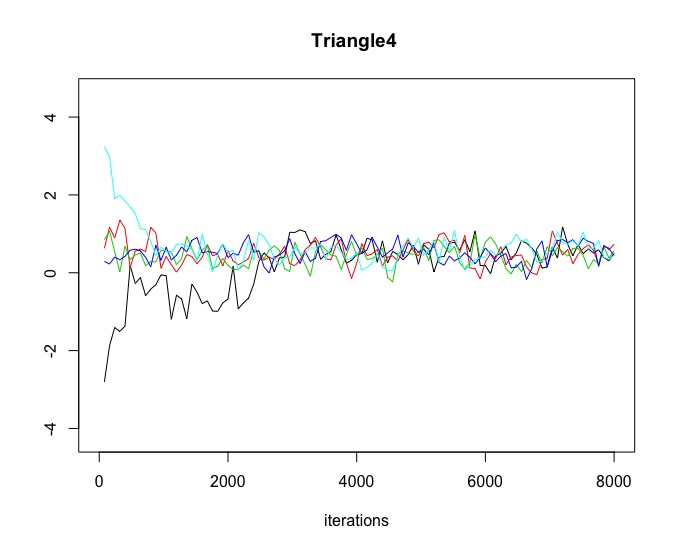
\includegraphics[scale=0.37]{Cap2/bayesTFR03.jpeg}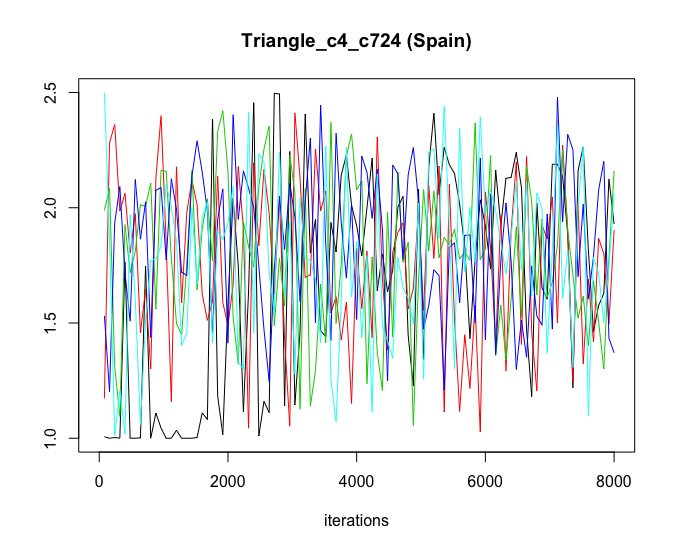
\includegraphics[scale=0.37]{Cap2/bayesTFR04.jpeg}
\captionsetup{width=1.05\linewidth}
\caption[Simulaciones del parámetro $\bigtriangleup$]{\textbf{Izquierda:} simulaciones de los parámetros MCMC para $\bigtriangleup_{4}$. \textbf{Derecha }simulaciones para el parámetro específico de España, $\bigtriangleup_{c4}$}
%\textit{(Fuente: World Bank World Development Indicators)}
\end{figure}

\noindent y por el comando\\ 

\vspace{-0.2cm}
{
\setlength{\fboxsep}{0.75pt}%
\noindent\setlength{\fboxrule}{0pt}%
\fbox{%
{\colorbox{gray!20}{\parbox{1\linewidth}{%
\small{\texttt{>\ tfr.partraces.cs.plot(country = "Spain", mcmc.list = m3, nr.points = 100,\\  
+ \hspace{0.5cm} par.names = "Triangle\_c4")}
}}}}}}}}\\

\noindent para el gráfico de la derecha $\bigtriangleup_{c4}$ específico de España.\\

\noindent También es posible visualizar las distribuciones de los hiperparámetros de la MCMC (\textbf{figura 2.7}), como hemos mencionado anteriormente y cuya equivalencia con el código en \textsf{\textbf{R}} se muestra a continuación:\\

\begin{tabular}{cccccccccccc}
 $\chi$ & \psi  &  \bigtriangleup_{4} &   $\alpha_{1,2,3}$ &  $\delta_{1,2,3}$   & $\delta_{4}$  & $\frac{exp(\alpha_{i})}{\sum_{j}exp(\alpha_{i})}$  & $a$  & $b$  & $S$  \\ \hline
\texttt{chi} & \texttt{psi} & \texttt{Triangle4} & \texttt{alpha} & \texttt{delta} & \texttt{delta4} & \texttt{alphat\_i} & \texttt{a\_sd} & \texttt{b\_sd} & \texttt{S\_sd} \\ 
\end{tabular}

\vspace{-0.2cm}
\begin{center}
\begin{tabular}{cccc}
$\sigma_{0}$ & c\textsubscript{1975} & $m_{\tau}$ & $s_{\tau} $\\ \hline
 \texttt{sigma0} & \texttt{cons\_sd} & \texttt{mean\_eps\_tau} & \texttt{sd\_eps\_tau}\\ 
\end{tabular}
\end{center}

\noindent El `script' utilizado viene dado por la función:\\

\vspace{-0.2cm}
{
\setlength{\fboxsep}{0.75pt}%
\noindent\setlength{\fboxrule}{0pt}%
\fbox{%
{\colorbox{gray!20}{\parbox{1\linewidth}{%
\small{\texttt{>\ tfr.pardensity.plot(pred2, par.names = c(``alphat", "Triangle4",  "delta",\\
+ \hspace{0.5cm} "sigma0"),  dev.ncol = 4, bw = 0.05)}
}}}}}}}}\\

\newpage
\vspace{-0.3cm}
\begin{figure}[!ht]
\centering
\hspace*{-0.1cm}
\includegraphics[scale=0.43]{Cap2/density.jpeg}
\caption{Densidad de las distribuciones de varios parámetros independientes del país}\\
%\textit{(Fuente: World Bank World Development Indicators)}
\end{figure}

\vspace{0.3cm}
Por otro lado la simulación también nos ha permitido calcular la TFR actual (\textbf{figura 2.8}) y las proyecciones (\textbf{figura 2.9}) a nivel mundial en cada país:

\begin{figure}[!htp]
\centering
\hspace*{0cm}
\includegraphics[scale=0.27]{Cap2/world01.png}
\caption{TFR 2010-2015 en cada país}\\
%\textit{(Fuente: World Bank World Development Indicators)}
\end{figure}

\begin{figure}[!htp]
\centering
\hspace*{-0.5cm}
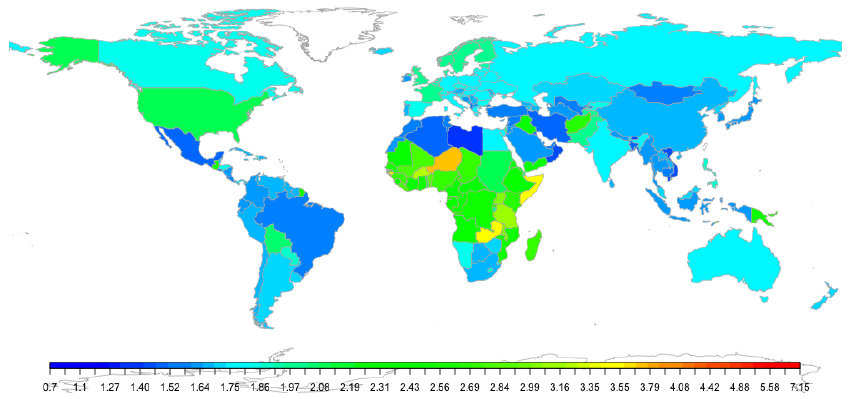
\includegraphics[scale=0.6]{Cap2/worldproj03.png}
\caption{Proyecciones de la TFR 2050-2055 en cada país}\\
%\textit{(Fuente: World Bank World Development Indicators)}
\end{figure}

Ello es porque en el paquete de simulación se ha incluido la posibilidad de crear mapas mundiales para cualquier periodo que se estime proyectar. Está hecho también con el software \textsf{\textbf{R}}, en concreto con los paquetes \textbf{`rworldmap'} (South, 2011 \textcolor{red}{[46]}) para el mapa y el paquete \textbf{`fields'} (Furrer y otros, (2011) \textcolor{red}{[47]}) para la leyenda de los gráficos.\\

Finalmente, también es posible simular las proyecciones mundiales de la TFR (\textbf{figura 2.10}) siguiendo la misma metodología que para el caso de España, dado que en las simulaciones que se han generado se han incluido, recordamos, 196 países, generándose pues, un fichero agregado que contiene las series históricas, especificadas por \'areas y continentes a nivel mundial. Si observamos el nivel proyectado de la TFR para el año 2050, situado ligeramente por encima de 2 nacimientos por mujer y lo comparamos con las proyecciones de la (\textbf{figura 2.3}), veremos que, efectivamente, coinciden. Gracias a las simulaciones hechas, esta forma de crear las proyecciones gráficas, tiene la ventaja de que se pueden generar mapas para proyectar otros periodos temporales sobre la misma escala.

\begin{figure}[!htp]
\centering
\hspace*{-1cm}
\includegraphics[scale=0.65]{Cap2/world02.png}
\captionsetup{width=1.1\linewidth}
\caption[Trayectoria de la TFR y distribución de la función logística doble]{\textbf{Izquierda:} trayectorias proyectadas de la TFR a nivel mundial. \textbf{Derecha:} distribuci\'on de la función logística doble.}}\\
%\textit{(Fuente: World Bank World Development Indicators)}
\end{figure}

\newpage
%-----------------------------------------  MODELOS DE MORTALIDAD ---------------------------------------------
\section{Modelos de predicción de la mortalidad: revisión y funcionamiento de los más usados}
%\hl{Mencionar a modo de introducci\'on el cap. 3 del libro ``Demograf\'ia: An\'alisis y Proyecciones''}.\\
Aunque la modelización de la mortalidad tiene una larga historia, concretamente desde que Benjamin Gompertz publicó su ley de la mortalidad en 1825, (Gompertz, 1825 \textcolor{red}{[48]}), numerosos modelos se han propuesto desde entonces, ya que los escenarios de mortalidad son una herramienta est\'andar en la proyecci\'on, entre otros, de los costes de beneficios definidos en los sistemas de pensiones basados en el reparto. Sin embargo, la predicci\'on de la mortalidad es un desafío más reciente. Solo hay que echar un vistazo a la \textbf{figura 2.11} y veremos que la mayoría de los modelos se han desarrollado en la última parte del siglo pasado y tan solo hace cuatro décadas los métodos que se usaban eran relativamente simples y estaban sujetos a un elevado grado de juicio subjetivo. Adem\'as, la tecnología de entonces imposibilitaba, en cierto modo, un análisis más sofisticado y aunque en los últimos veinte años se han desarrollado y aplicado metodologías más complejas, estos modelos, en general, no han utilizado métodos desarrollados principalmente para la graduación específica por edad. En vez de eso, los actuarios y los demógrafos han hecho uso cada vez mayor de métodos estadísticos estándar.

\begin{figure}[!htp]
\centering
\fbox{\includegraphics[scale=0.3]{Cap2/modelhist.png}}
\captionsetup{width=1.1\linewidth}
\caption{Línea temporal de la aparición de los modelos de mortalidad}\\
{\small{\textit{Fuente: Pascariu y Canudas-Romo (https://www.mortality.org/Public/HMD\_4th\_Symposium/Pascariu\_poster.pdf)}}}
\end{figure}


Las proyecciones de vida y financieras que iluminan el estado financiero de los sistemas de pensiones son, indiscutiblemente importantes, no solo porque los sistemas de reparto transfieren recursos considerables de los trabajadores a los jubilados, sino porque las proyecciones de vida se usan para calcular las pensiones individuales. A medida que aumenta la esperanza de vida, y asumiendo los patrones actuales de jubilaci\'on, entre el 35 y el 40 por ciento de la población total en la OCDE ser\'an jubilados dentro de las pr\'oximas tres d\'ecadas.\\

Constantemente asistimos a publicaciones oficiales que proporcionan una imagen de las contribuciones y pagos futuros en función de diversos escenarios demográficos y económicos. Estos informes proporcionan una visión del desarrollo financiero de los sistemas nacionales de pensiones.\\

El debate que surge en pa\'ises de todo el mundo sobre c\'omo hacer frente al envejecimiento de la poblaci\'on no es nuevo, ya venimos se\~nalando que cada vez son m\'as las voces que se alzan (en la figura de diferentes colectivos, p\'ublicos y privados), poniendo de manifiesto la insuficiencia de los gobiernos para hacer frente a los diferentes fen\'omenos demogr\'aficos (longevidad, fertilidad y migración) que est\'an modificando la estructura de muchos pa\'ises. En este sentido, la publicaci\'on del informe de investigaci\'on del Banco Mundial \textcolor{red}{[49]}, constituy\'o un hito en el debate. Este organismo, recomend\'o que sus pa\'ises clientes adoptaran esquemas de varios pilares, con un ``segundo pilar'' financiado que juega un papel importante.\\

Para predecir la poblaci\'on debemos complementar los pron\'osticos de mortalidad con pron\'osticos similares para la fertilidad y si es necesario, para la inmigraci\'on. Estos elementos se pueden combinar en el procedimiento habitual de componentes de cohorte para generar predicciones estoc\'asticas de la misma, aunque los pron\'osticos de fertilidad plantean desaf\'ios especiales ya que no parece haber un patr\'on temporal `fuerte' para estas din\'amicas.\\

De esta forma, la mayoría de los análisis de la evolución histórica de las tasas de mortalidad se hacen usando modelos que descomponen dichas tasas de mortalidad en las dimensiones de edad, período y cohorte (o año de nacimiento). Estas tres variables forman una manera natural de analizar cómo cambian las tasas de mortalidad para las personas a medida que envejecen, el impacto del progreso médico y social con el tiempo y los efectos de la mortalidad a lo largo de la vida que siguen a las personas desde el nacimiento. Al proyectar los efectos del período y la cohorte, también se puede obtener información sobre la posible trayectoria que las tasas de mortalidad podrían seguir en el futuro.\\

Con los avances de la informática y las herramientas computacionales, las posibilidades de modelizar y examinar varios supuestos son hoy en día, más o menos, ilimitadas. La introducción de métodos estocásticos tiene la gran ventaja de producir una predicción de la distribución de probabilidad en vez de un pronóstico puntual determinista. Esta es la línea de trabajo, por ejemplo, de Juha Alho, el cual argumenta que tradicionalmente, el problema de cómo anticipar mejor los pronósticos demográficos que se hacen para el futuro surgen, naturalmente, en un entorno de sostenibilidad fiscal, es decir, sólo en este contexto, los responsables y administradores políticos hacen los análisis bajo suposiciones de que los futuros cambios demográficos son deterministas. En base a esto, el autor, afirma que si se considerase una demografía estocástica tales problemas se simplificarían porque los reguladores políticos basarían sus decisiones en las predicciones de la población futura pero revisarían esas decisiones cuando resulte que la demografía no sigue el camino esperado (Alho, 1990, \textcolor{red}{[50]}; Alho y Spencer, 2005 \textcolor{red}{[51]}).\\

Por regla general, la predicción de la mortalidad implica la especificación de un modelo subyacente de los datos y de un modelo de previsión. Estos modelos pueden ser distintos o integrados en un marco único. Así, se suelen emplear tres variables o factores: edad, período (o tiempo) y cohorte para clasificar el modelo subyacente como cero, uno, dos o tres (Tabeau, 2001) \textcolor{red}{[52]}. Los \textit{modelos de factor 0} son simplemente una medida agregada o una tasa específica por edad (donde cada edad se trata de forma independiente); en este caso, no hay un modelo subyacente especificado. Los \textit{modelos de un solo factor} tratan las tasas de mortalidad (período o cohorte) como una función de la edad, lo que permite aprovechar su regularidad a lo largo de la edad y, al pronosticar, la estabilidad de los patrones a lo largo del tiempo. Los \textit{modelos de dos factores} normalmente, tienen en cuenta la edad y el período, por ejemplo, los métodos más recientes de predicción de la mortalidad emplean tales modelos. Los \textit{modelos de tres factores} (o APC, \textit{Age-Period-Cohort}) expresan las tasas en función de la edad, el período y la cohorte.\\

La mayoría de los métodos de predicción de la mortalidad son por extrapolación; es decir, hacen uso de la regularidad que, típicamente, se encuentra en ambos patrones de edad y de tendencias a lo largo del tiempo. Este enfoque incluye la extrapolación tradicional y `relativamente' simple de medidas agregadas, como la esperanza de vida, así como métodos más complejos. En este sentido, el método Lee--Carter, ha sido el primer (y todavía más usado), modelo de mortalidad de estructura \textsc{apc} (Lee y Carter, 1992 \textcolor{red}{[53]}). En él, los autores proponen un modelo de la forma $$ln(\mu_{x,t})=\alpha_{x}+\beta_{x}\kappa_{t}+\varepsilon_{x,t},$$ es decir, con un solo término edad/periodo y modelizan el logaritmo de la mortalidad, $\mu_{x,t}$, ajustando el modelo mediante el uso de un proceso de dos etapas: en la primera etapa se estiman los parámetros utilizando la descomposición de valores singulares, que es una aplicación de los métodos de ajuste de mínimos cuadrados para una estructura de predicción bilineal, y en la segunda etapa se ajusta $\kappa_{t}$ para ajustar mejor el número observado de muertes en cada año. Wilmoth (1993) \textcolor{red}{[54]} y Lee (2000) \textcolor{red}{[55]}, adaptaron este enfoque de dos etapas pero conservando el uso de la estimación por métodos cuadrados.\\

Más tarde, Booth y otros, (2002) \textcolor{red}{[56]}, fueron los primeros en señalar que el uso de descomposición de valores singulares para ajustarse al modelo Lee-Carter, selecciona solo el primero de un número potencialmente grande de términos de edad/periodo, por lo tanto, el modelo se extendió a una forma más compleja del tipo $$ln(\mu_{x,t})=\alpha_{x}+\sum_{i=1}^{N}\beta_{x}^{(i)}\kappa_{t}^{(i)},$$ derivándose un modelo de dos términos, comúnmente referido como modelo LC2\footnote{LC por Lee-Carter.} 
$$ln(\mu_{x,t})=\alpha_{x}+\beta_{x}^{(1)}\kappa_{t}^{(1)}+\beta_{x}^{(2)}\kappa_{t}^{(2)},$$

\noindent el cual ha sido estudiado en detalle por Renshaw y Haberman, (2003) \textcolor{red}{[57]}.\\

En consecuencia, extensiones al modelo de Lee-Carter, han proliferado desde entonces, por ejemplo, Hyndman y Ullah (2007) \textcolor{red}{[58]}, exploraron modelos con múltiples términos edad/periodo y usaron el análisis funcional de datos para ajustar estos modelos; Hatzopoulos y Haberman (2009) \textcolor{red}{[59]}, usaron modelos lineales generales y Wang y otros (2009) \textcolor{red}{[60]}, emplearon el uso de análisis de componentes principales. Sin embargo, ninguna de estas extensiones al modelo LC original se han mostrado menos populares de lo esperado en la práctica, posiblemente debido a que las funciones de orden superior muestran un comportamiento complicado, cuyos cambios en la tendencia dificultan hacer predicciones.\\

En 2006, Cairns, Blake y Dowd introdujeron el modelo que lleva su nombre, CBD, (Cairns y otros, 2006 \textcolor{red}{[61]}), para para superar el problema de que las tasas de mortalidad proyectadas estén perfectamente correlacionadas en los modelos de una sola edad/período. Competidor directo del modelo de Lee-Carter, el modelo CBD es de la forma $$logit(q_{x,t})=\kappa_{t}^{(1)}+(x-\overline{x})\kappa_{t}^{(2)},$$ resaltando los autores dos características: la ausencia  de la función de edad estática $\alpha_{x}$, la cual reduce el número de parámetros libres, obteniéndose así un modelo más `moderado' y el uso de una función logit como elementos diferenciadores del enfoque del modelo CBD en contraposición de los modelos basados en el estilo LC.\\

Así, en una generalización del modelo CBD, Cairns y otros (2009) \textcolor{red}{[62]} proponen la forma $$logit(q_{x,t})=\sum_{i=1}^{N}\beta_{x}^{(i)}\kappa_{t}^{(i)}\gamma_{t-x}^{(i)},$$ y posteriormente y en base a lo anterior, en Cairns y otros (2011) \textcolor{red}{[4]}, los autores desarrollan un marco de trabajo donde analizan y desarrollan seis modelos estocásticos de mortalidad (de ocho propuestos) de la forma:

\vspace{-0.4cm}
\begin{center}
{
\extrarowsep=2ex
\begin{tabular}{ll}
Modelo & Fórmula \\ \hline
M1 & $log\ m(t,x)=\beta_{x}^{(1)}+\beta_{x}^{(2)}\kappa_{t}^{(2)}$\\ 
M2 & $log\ m(t,x)=\beta_{x}^{(1)}+\beta_{x}^{(2)}\kappa_{t}^{(2)}+\beta_{x}^{(3)}\gamma_{t-x}^{(3)}$\\
M3 & $log\ m(t,x)=\beta_{x}^{(1)}+n{a}^{-1}\kappa_{t}^{(2)}+n{a}^{-1}\gamma_{t-x}^{(3)}$\\
M5 & $logit\ q(t,x)=\kappa_{x}^{(1)}+\kappa_{x}^{(2)}(x-\overline{x})$\\
M7 & $logit\ q(t,x)=\kappa_{x}^{(1)}+\kappa_{x}^{(2)}(x-\overline{x})+\kappa_{x}^{(3)}((x-\overline{x})^{2}-\hat{\sigma}^{2}_{x})+\gamma_{t-x}^{(4)}$\\
M8 & $logit\ q(t,x)=\kappa_{x}^{(1)}+\kappa_{x}^{(2)}(x-\overline{x})+\gamma_{t-x}^{(3)}(x_{c}-x)$\\ \hline
\end{tabular}
}
\end{center}

\vspace{0.3cm}
El problema del modelo clásico APC es que su ajuste se hace usando el método de mínimos cuadrados ordinarios, ya que el modelo es lineal en los parámetros; sin embargo, esto conlleva la construcción de una matriz, la cual es singular y por lo tanto no puede ser invertida tal y como requiere el enfoque de mínimos cuadrados. Esta singularidad, causada por la falta de identificabilidad de los parámetros en el modelo APC ha generado una abundante literatura sobre diferentes métodos para intentar un buen ajuste del modelo, como se puede comprobar en Glenn (1976) \textcolor{red}{[63]}, Fienberg y Mason (1979) \textcolor{red}{[64]}, Rodgers (1982) \textcolor{red}{[65]}, Holford (1983) \textcolor{red}{[66]}, Wilmoth (1990) \textcolor{red}{[67]}, Kuang y otros (2008) \textcolor{red}{[68]},  O'Brien (2011) \textcolor{red}{[69]} y Currie (2016) \textcolor{red}{[70]}.\\

Todos estos métodos propuestos no dejan de ser híbridos, tal y como señalan Hunt y Blake (2015) \textcolor{red}{[71]}, con combinaciones de las características de los modelos de Lee-Carter, de Cairns-Blake-Dowd y el modelo APC.\\

Por otro lado, Lee y Tuljapurkar (1994) \textcolor{red}{[72]}, usan modelos de series de tiempo para hacer pronósticos estocásticos para la población de los EEUU; Giacometti y otros (2012) \textcolor{red}{[73]}, comparan el modelo Lee-Carter y el modelo AR-ARCH a la hora de predecir las tasas de mortalidad, proponiendo este último como alternativa y concluyendo que el modelo AR(1)-ARCH(1) con una \textit{t}-Student proporciona un mejor ajuste. \\

Otro enfoque, en cambio, considera el problema de conciliar los pronósticos de tasa de mortalidad específica por edad desde el punto de vista de los métodos de pronóstico de series temporales univariadas agrupadas (Hyndman, Ahmed y otros, 2011 \textcolor{red}{[74]}) y lo extienden a las series temporales funcionales (Shan y Hyndman, 2016 \textcolor{red}{[75]})\\ 

Hunsinger (2014) \textcolor{red}{[76]}, también propone una predicción estocástica de la población usando modelos autorregresivos con coeficientes aleatorios. En concreto propone modelos para la fertilidad, la mortalidad y la migración y Ekheden y H\"osjer (2015) \textcolor{red}{[77]}, introducen un modelo de regresión mixta para datos de mortalidad que se puede descomponer en un componente de tendencia determinista y que viene explicado: por las covariables edad y año, por una parte de la serie temporal gaussiana multivariante no explicada por las covariables anteriores y por y el riesgo binomial. Los autores ajustan los datos de mortalidad para los Estados Unidos y Suecia.\\
 
Por su parte, Kleinow y Richards (2017) \textcolor{red}{[78]}, también en esta línea, muestran que los modelos ARIMA se ajustan mejor para representar las series temporales de la mortalidad que los modelos basados en paseos aleatorios.\\

Keilman y Pham, (2004) \textcolor{red}{[79]}, han ampliado considerablemente sus modelos simples y sugieren varias formas de modelar y limitar la volatilidad de los pronósticos de proyección de la población.\\
 
Otro tanto hacen Neves y otros (2017) \textcolor{red}{[80]} cuando amplían el modelo de Lee-Carter utilizando una nueva clase de modelos de series temporales, conocidos como modelos de Puntuación Generalizada Autorregresiva (GAS) o Puntuación Condicional Dinámica (DCS). Este marco puede usarse para derivar una amplia gama de modelos de series temporales no-gaussianas con coeficientes que varían en el tiempo. Así, proponen cinco modelos de probabilidad (Poisson, binomial, binomial negativo, gaussiano y beta) basados en el modelo GAS para estimar los parámetros de Lee-Carter y pronosticar, dinámicamente, las tasas de mortalidad usando un solo paso unificado. Los modelos se aplican a las series temporales de tasas de mortalidad para la población masculina de los Estados Unidos, Suecia, Japón y el Reino Unido.\\

Un enfoque más explicativo a la hora de proyectar la mortalidad, hace uso de modelos estructurales o epidemiológicos de mortalidad de ciertas causas de muerte, donde se conocen las variables exógenas clave y se pueden medir; finalmente, en un tercer enfoque (de expectativas), las previsiones se basan en las opiniones subjetivas de expertos que involucran diversos grados de formalidad.\\

El trabajo de Calian y Har\dh\ \hspace{-0.12cm}son, (2015) \textcolor{red}{[81]}, por ejemplo, est\'a en l\'inea con lo anteriormente citado. En su investigaci\'on, las predicciones est\'an basadas en la aplicaci\'on de m\'etodos estad\'isticos y modelos de componente de cohorte para proyecciones de poblaci\'on anuales, a corto y a largo plazo y mediante el análisis de series temporales con datos de migraciones, nacimientos y muertes, construyen modelos que usan para calcular puntos e intervalos de confianza estimados para predecir los componentes de la población.\\

Una de las consideraciones fundamentales a la hora de pronosticar la mortalidad es la medida a pronosticar, la cual depende del \textit{propósito de la predicción y de la disponibilidad de los datos} (Booth y Tickle, 2008) \textcolor{red}{[82]}. En la mayoría de los casos, las tasas (o probabilidades) de mortalidad según el sexo son de interés primordial, junto a las correspondientes tablas de vida derivadas. Cuando sólo se pronostica la esperanza de vida, lo más habitual en el caso de países en vías de desarrollo,  se puede utilizar una tabla de vida modelo adecuada para proporcionar detalles específicos de la edad. Cuando lo que es relevante es el número de muertes, se derivan mejor de las tasas de mortalidad pronosticadas a través del pronóstico de la población (Booth, 2006) \textcolor{red}{[83]}.\\

Los hallazgos empíricos del uso del modelo de Lee-Carter y sus extensiones optan por un modelo \textit{ARIMA (p,1,q)} para modelizar la dinámica de los logaritmos de las tasas de mortalidad, lo que se denomina índice de mortalidad siendo un elemento clave para pronosticar y evaluar dichas tasas y gestionar el riesgo de longevidad. Sin embargo, según Leng y Peng, tanto el modelo de Lee-Carter como sus extensiones, no pueden detectar la verdadera dinámica del índice de mortalidad en general, lo que significa que las proyecciones de mortalidad futuras basadas en el procedimiento de inferencia de dos pasos en este modelo son cuestionables (Leng y Peng, 2016 \textcolor{red}{[84]}).\\

En la misma línea crítica con el modelo de Lee-Carter se mueven Mitchell y otros (2013) \textcolor{red}{[85]}, los cuales proponen un modelo que analiza los datos de mortalidad desde una perspectiva diferente, mostrando que al realizar primero una transformación simple de los datos antes de modelizar, dicha modelización posterior mejora, considerablemente, la capacidad para replicar la dinámica de las tasas de mortalidad a través del tiempo.\\

También Wang, Jack Yue y Chong expresan sus objeciones al modelo de Lee-Carter cuando se trata de aplicarlo a poblaciones pequeñas, afirmando que se obtienen resultados poco satisfactorios para esos casos, proponiendo, en cambio un enfoque alternativo basado en una combinación de datos agregados y graduación de la mortalidad (Wang y otros, 2018 \textcolor{red}{[86]}).\\

Al igual que veíamos en la sección de los modelos de fertilidad, la estadística bayesiana también ha sido empleada en la modelización y proyección de la mortalidad. As\'i, Wi\`sniowski, Smith y otros, (2015) \textcolor{red}{[87]} desarrollan una aproximación bayesiana integrada y dinámica que incorpora los modelos tipo Lee-Carter para pronosticar los patrones de edad, con medidas asociadas de incertidumbre, de fertilidad, mortalidad, inmigración y emigración dentro de un modelo de proyección de cohorte. Sin embargo, los inconvenientes del modelo de Lee-Carter y sus derivados, hacen que estos mismos autores se centren en uno de los inconvenientes del modelo de Poisson Lee-Carter que impone la igualdad entre la media y la varianza y restringe las variaciones de mortalidad entre los individuos, presentando dos modelos para explicar potencialmente la sobredispersión y ajustándolos en un marco bayesiano (Wong, Forster y Smith, 2017, \textcolor{red}{[88]}).\\

Alexander y otros (2017) \textcolor{red}{[89]}, consideran esencial la estimación de la mortalidad sub-nacional en el estudio de las desigualdades en la salud dentro de un país. De esta forma y al igual que vimos anteriormente en Wang y otros (2018) \textcolor{black}{[86]}, en la línea de la aplicación de los modelos de mortalidad a poblaciones pequeñas, los autores presentan un modelo jerárquico bayesiano para estimar la mortalidad a nivel subnacional. El modelo se basa en los patrones de edad característicos de las curvas de mortalidad, que se construyen utilizando componentes principales de un conjunto de curvas de mortalidad de referencia.\\ 

Lin y O'Hare, (2017) \textcolor{red}{[90]} proponen un modelo de mortalidad con coeficiente de variación en el tiempo (TVC) que apunta a combinar las buenas características de los modelos existentes con métodos de calibración de modelos eficientes, aplicando técnicas no paramétricas de suavizado y Hilton y otros, (2018) \textcolor{red}{[91]}, también dentro del enfoque paramétrico, presentan un enfoque bayesiano para el pronóstico de la mortalidad que calcula conjuntamente un modelo aditivo generalizado (GAM) para la mortalidad en la mayor parte del rango de edad y un modelo paramétrico para las edades mayores donde los datos son más escasos.\\

Autores como Fung, Peters y Shevchenko abordan el problema de la modelización de la mortalidad con factores de cohorte incorporados, a través de una nueva formulación bajo una metodología de espacio de estado,\footnote{Un \textbf{modelo de espacio de estados} es un modelo matemático de un sistema físico descrito mediante un conjunto de entradas, salidas y variables de estado relacionadas por ecuaciones diferenciales de infinito orden que se combinan en una ecuación diferencial matricial de primer orden.} demostrando que los factores de cohorte se pueden formular de manera natural en el marco del espacio estatal, a pesar de que los factores de cohorte se indexan según el año de nacimiento en lugar del año (Fung, Peters y Shevchenko, 2018, \textcolor{red}{[92]}).\\ 

Otros investigadores como Rabbi y Mazzuco comparan y contrastan los modelos de pronóstico de mortalidad para regímenes de mortalidad más altos en países que carecen de datos de series cronológicas de buena calidad, lo cual es común en varios países de Europa Central y Oriental para ello, utilizan siete variantes diferentes del método de Lee-Carter, los pronósticos coherentes de mortalidad de varios países de Europa central y oriental y el modelo jerárquico bayesiano utilizado por las Naciones Unidas para producir predicciones probabilísticas, considerando los datos de nueve países de Europa con una mortalidad comparativamente más alta, como por ejemplo Bielorrusia, Rusia, Ucrania o Hungría, llegando a la conclusión de que los hallazgos obtenidos implican la necesidad de crear nuevas técnicas de predicción para países con un elevado índice de mortalidad (Rabbi y Mazzuco, 2018, \textcolor{red}{[93]}).\\

Como se ha mencionado anteriormente, la proyección de la mortalidad como parte del riesgo de longevidad tiene un impacto crucial en las políticas sociales y económicas de los gobiernos. Todas las evaluaciones cuantitativas de la sostenibilidad fiscal que incluyen los efectos del envejecimiento de la población deben utilizar pronósticos demográficos. Es bien sabido que tales pronósticos son inciertos, y algunos estudios lo han tenido en cuenta al utilizar proyecciones de población estocásticas conjuntamente con modelos económicos. La comunidad investigadora y científica también ha centrado sus investigaciones en esta vertiente buscando siempre cuantificar y minimizar el impacto de ese riesgo de longevidad; Lassila, Valkonen y Alho (2014) \textcolor{red}{[94]}, desarrollan este enfoque mediante la introducción de revisiones periódicas de los pronósticos demográficos que están integradas en las proyecciones estocásticas de la población. Según los autores, esto permite separar, para cada resultado demográfico y bajo diferentes reglas de política, los efectos esperados y realizados del envejecimiento de la población en las finanzas públicas.\\

Wills y Sherri (2011)  \textcolor{red}{[95]}, por su parte, desarrollan un modelo de longevidad estocástico adecuado para aplicaciones de precios y gestión de riesgos basadas en las tasas de mortalidad de la población australiana de 1971 a 2004 para las edades de 50 a 99 años. El modelo permite los cambios esperados que surgen de la edad y los efectos de la cohorte e incluye múltiples factores de riesgo estocásticos. Asímismo, captura los efectos de la edad y el tiempo y permite la dependencia de la edad en los factores estocásticos que impulsan las mejoras de la longevidad. Los autores concluyen que el modelo proporciona una buena adaptación a los datos históricos que capturan las tendencias estocásticas en la mejora de la mortalidad en diferentes edades y en el tiempo, así como la estructura de dependencia multivariable a través de las edades.\\

M\"a\"att\"anen y Alho (2014) \textcolor{red}{[96]}, exponen los inconvenientes de las proyecciones demográficas en el sentido de que la evidencia histórica muestra que dichas predicciones, incluyendo las predicciones de la mortalidad, a menudo han sido más erróneas de lo que se suele creer; como consecuencia de esto, dichos pronósticos tienden a actualizarse con bastante frecuencia. Los autores discuten este problema desde el punto de vista del ahorro en el ciclo de vida y de la oferta laboral en el que una cohorte de trabajadores decide cuánto trabajar y cuánto ahorrar para las pensiones. Siguiendo en el contexto de una mortalidad estocástica, los pronósticos puntuales se actualizan periódicamente y los autores derivan una aproximación markoviana para la distribución predictiva de la mortalidad y permite comparar una solución de expectativas racionales teóricamente óptima con una estrategia en la que la cohorte simplemente actualiza el plan de ciclo de vida para que coincida con cada pronóstico de mortalidad actualizado.\\

Holzmann, Villegas y otros, (2017) \textcolor{red}{[97]}, encuentran evidencias empíricas de que entre países, la longevidad es altamente heterogénea en características socioeconómicas clave, incluidos los ingresos. Una relación positiva entre los ingresos y la expectativa de vida en la jubilación equivale a un mecanismo directo de impuestos/subsidios cuando se aplica la expectativa de vida de la cohorte promedio para el cálculo de la anualidad, como se hace bajo los esquemas de contribución no financiera definida (Non-Defined Contribution). Dicha redistribución regresiva y la consiguiente distorsión del mercado laboral ponen en duda las características principales del esquema de contribución no definida y exige diseños de beneficios alternativos para compensar la heterogeneidad. De esta forma, los autores exploran cinco mecanismos clave de compensación: anualidades individualizadas; tasas de contribución individualizadas/asignaciones de cuentas; una estructura de contribución de dos niveles con estructura de tarifas socializada e individual; y dos enfoques complementarios bajo el enfoque de dos niveles para tratar las colas de distribución de ingresos y las distorsiones por encima y por debajo de un determinado nivel. Usando datos de Inglaterra, Gales y Estados Unidos, concluyen que tanto las anualidades individualizadas como un esquema de contribución de dos niveles son factibles y efectivos, siendo opciones políticas prometedoras.\\

Para el caso de nuestro país, cabe mencionar el trabajo de Amancio Beztuen, quien, contrastando la validez del modelo de Lee-Carter, primero y seleccionando, posteriormente, un intervalo factible para la validez de la proyección, ha aplicado el estudio para la población española (ambos sexos), contrastando el resultado y proyectándolo hasta el año 2030, concluyendo que cuando se elige adecuadamente el colectivo así como el horizonte temporal, el modelo de Lee-Carter proporciona unos buenos resultados, siendo la regresión lineal una buena estimación hacia el futuro, sin embargo, en palabras del autor: \textit{``el modelo no proporciona los mismos resultados en cuanto a la esperanza matem\'atica de vida a partir de los 65 a\~nos, cuando se toma en consideración todo el grupo de edades desde la edad inicial hasta la edad l\'imite superior biom\'etrico''} (Beztuen, 2010 \textcolor{red}{[98]}).\\

Por su parte, Benchimol, 2017 \textcolor{red}{[99]}, presenta una metodología para elaborar tablas de mortalidad dinámicas y proporcionar una herramienta para poder cuantificar el impacto económico del riesgo de longevidad. Dicha metodología, reúne los modelos de mortalidad más usuales y proyecta las tasas de mortalidad de España por medio de una mixtura de los mismos basada en el criterio de información de Akaike, concluyendo que mediante intervalos de predicción al 95\%, la mixtura de modelos ha sido capaz de proyectar correctamente las tasas centrales de mortalidad en la gran mayoría de los casos, con menor sesgo y/o mayor precisión que los modelos considerados individualmente sobre el mismo conjunto de datos.

%----------------------------------------------------------------------------------------
%\newpage

%\subsection{Algunas simulaciones con \textsf{R}: mortalidad, esperanza de vida y brecha de mortalidad}
\subsection{Predicción en la poblaci\'on espa\~nola con los paquetes `MortalityLaws', `MortalityGap' y `StMoMo'}

La extensa literatura en materia de modelos de pronóstico y predicción de la mortalidad dificulta la idea de abarcar una revisión pormenorizada y exhaustiva, provocando que, tras hacer un análisis lo más actualizado y variado de las diferentes metodologías aplicadas, nos detengamos para continuar hacia adelante y pasar a centrarnos en nuestro país de forma que, del mismo modo que hicimos en el apartado 2.2.1 cuando usamos un modelo para proyectar la fertilidad española, procedemos del mismo modo para varios análisis; por un lado, la intención es establecer la relaci\'on entre la tasa bruta de mortalidad y la esperanza de vida, mediante una simulación/comparación entre varios países, a continuación, usaremos un modelo para la proyección de la esperanza de vida pero diferenciando entre sexo y finalmente, adaptaremos un modelo estocástico de mortalidad para la población española.\\

Hemos creído conveniente comenzar viendo la relación entre la tasa bruta de mortalidad y la esperanza de vida. Como se puede ver en la \textbf{figura 2.12}, con los datos disponibles, hemos representado desde 1960 hasta 2016 este ratio, observando que dicha tasa ha pasado de una tasa mortalidad bruta de algo más de 8,5 por cada mil habitantes para una esperanza de vida de algo menos de 70 años, hasta situarse en menos de 9 con una esperanza de vida de 82 años, aproximadamente. Entre estos dos periodos, como se observa en la gráfica, la tasa de mortalidad se ha estado moviendo, más o menos, entre 8 y 9, a medida que incrementaba la esperanza de vida, considerándose bastante estable en estos últimos 60 años, si bien podemos destacar períodos  puntuales en los que la tasa de mortalidad disminuyó y aumentó; con todo, se puede considerar una tasa bruta de mortalidad bastante estable, sin olvidar que el incremento en la esperanza de vida ha sido considerable.\\

\begin{figure}[!htp]
\centering
\hspace*{-1cm}
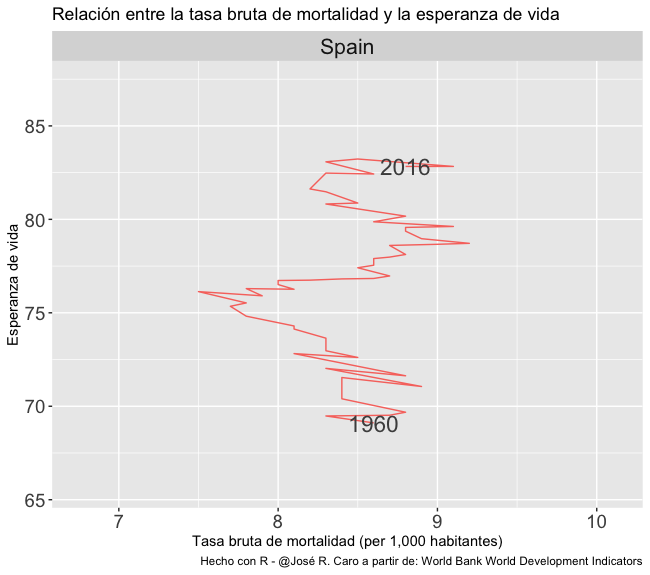
\includegraphics[scale=0.4]{Cap2/lifeexpspain.png}
\caption{Relaci\'on entre la tasa de mortalidad y la esperanza de vida en España}\\
\textit{(Fuente: Elaboración propia a partir de World Bank World Development Indicators)}
\end{figure}

Lo interesante de este análisis es comparar España con otros países, ya que si podemos considerar que durante los últimos 60 años España ha gozado de cierta estabilidad en cuanto una tasa bruta de mortalidad `contenida' mientras la esperanza de vida no ha dejado de crecer, podría ser conveniente ver qué ocurre con esta misma relación en otros países, no ya del entorno o del mismo continente que España, sino a nivel mundial. Para ello, como se puede apreciar en la \textbf{figura 2.13}, hemos seleccionado doce países, algunos de ellos con un índice de desarrollo por debajo del normal, para ver cómo ha evolucionado tanto la tasa bruta de mortalidad como la esperanza de vida. De este modo, hemos hecho seleccionado a Mozambique, Etiopía y Zambia como representativos del continente africano, observando en todos ellos que la tasa bruta de mortalidad ha disminuido en proporciones considerables (si bien estaba en unos índices muy elevados) y la esperanza de vida ha aumentado, también de forma importante, como cabría esperar, si bien en estos países la mejora es más acentuada, pues venían de una situación de extrema gravedad. Particularmente llamativo es el caso de Zambia ya que se observa que la relación entre la tasa bruta de mortalidad y la esperanza de vida retrocede en un periodo que va desde principios de la década de los 80 hasta mediados de los 90, durante este tiempo, la esperanza de vida que llegó a ser de 52 años en 1980, retrocedió hasta casi los 40 años y cuya explicación la encontramos en los altos niveles de pobreza y las enfermedades como la malaria, la tuberculosis y el VIH que asolaron el país y provocaron las muertes prematuras de millones de zambios.\\

La inclusión de India, China y Japón se debe a que son los países asiáticos más importantes y de mayor crecimiento en cuanto a  población se refiere en los últimos años y los dos primeros se comportan de forma parecida a los países africanos mencionados antes, es decir, han pasado de tener una tasa de mortalidad bruta `relativamente' alta y una esperanza de vida bastante baja, a disminuir, de forma ostensible la primera y a incrementar, de forma considerable, la segunda. Destacable es el caso de Japón, uno de los países donde la esperanza de vida es más alta pero a la vez más envejecida, por ello experimenta un incremento en ambas magnitudes.\\

Similar comportamiento (descenso abrupto de la tasa de mortalidad e incremento progresivo de la esperanza de vida) podemos apreciar en México, Brasil y Chile, como países seleccionados de América Central y del Sur aunque parten de una situación mejor, con unas tasas bruta de mortalidad inferiores y una esperanza de vida mayores que los anteriores países, finalmente, ya dentro de los países más desarrollados, hemos creído conveniente incluir a los Estados Unidos, Australia y Canadá, los cuales tienen un comportamiento `parecido' a España.


\newpage

\begin{figure}[!htp]
\centering
\hspace*{-1.3cm}
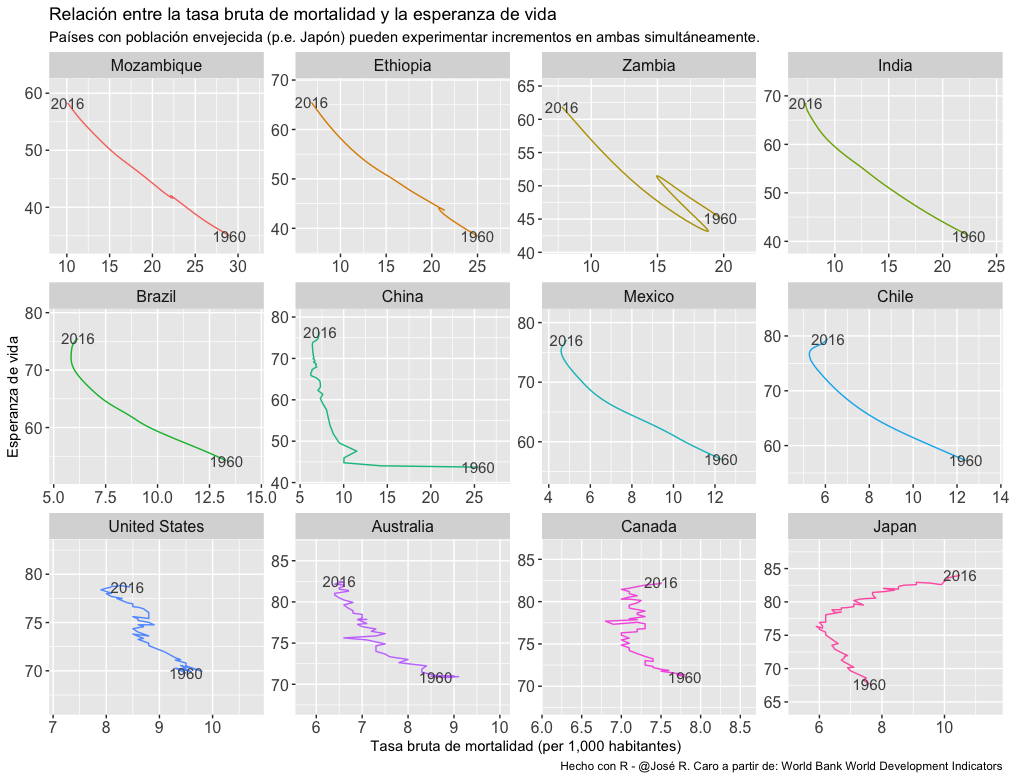
\includegraphics[scale=0.53]{Cap2/relactasaesp.png}
\captionsetup{width=1.1\linewidth}
\caption{Relaci\'on entre la tasa de mortalidad y la esperanza de vida en algunos países seleccionados}\\
\textit{(Fuente: Elaboración propia a partir de World Bank World Development Indicators)}
\end{figure}

La importancia del análisis anterior radica en que la perspectiva comparada entre países nos permite ver la estrecha relación entre tasa bruta de mortalidad e incremento de esperanza de vida que se produce tanto en países subdesarrollados o en vías de desarrollo como en países más avanzados; por otro lado, nuestro país, nos sitúa en un buen punto de partida para introducir las proyecciones de la mortalidad que a continuación desarrollaremos y que como indicamos al principio del tema, están basadas en los modelos estocásticos de mortalidad  de \textsc{E}dad/\textsc{P}eriodo/\textsc{C}ohorte (Age/Period/Cohort), que incluyen los ya mencionados modelos de Lee-Carter y Cairns-Blake-Dowd, ya que aún hoy, a pesar de las críticas suscitadas, los inconvenientes señalados y las modificaciones y mejoras aportadas, estos modelos siguen siendo de los más usados a la hora de proyectar la mortalidad. Concretamente, como señalan Girosi y King (2007) \textcolor{red}{[100]}, el modelo de Lee-Carter posee varias características no reconocidas o insuficientemente apreciadas, por lo que la investigación de dichos autores, podría ser una buena aproximación para entender el modelo que Ronald Lee y Lawrence Carter crearon en 1992.\\

Ya hemos hecho mención anteriormente a la estructura de los modelos de \textsc{E}dad/\textsc{P}eriodo/\textsc{C}ohorte (en adelante y para estar en línea con la nomenclatura anglosajona y evitar confusiones, lo denominaremos APC) y decíamos que un modelo de mortalidad de esta estructura es aquel que vincula una variable de respuesta con una estructura de predictor lineal o bilineal, que consiste en una serie de factores que dependen de la edad, $x$, período, $t$ y año de nacimiento (o cohorte), $y = t - x$, para una población. Por lo tanto, los modelos APC se encajan en la clase general de modelos no lineales generalizados, con una estructura que se puede describir como sigue: $$\eta_{x,t}=\alpha_{x}+\sum_{i=1}^{N}\beta_{x}^{(i)}\kappa_{t}^{(i)}+\beta_{x}^{(0)}\gamma_{t-x}$$
cuyos componentes quedan definidos:

\begin{itemize}[label={\Large\textbullet}]
\item Una función de enlace, $\eta_{x,t}$, para transformar la variable de respuesta (que será una medida de las tasas de mortalidad) a la edad $x$ y para el año $t$ en una forma adecuada para modelizarla y vincularla a la estructura del predictor propuesta.
\item Una función de edad estática, $\alpha_{x}$, para capturar la forma general de la mortalidad en todas las edades y características de la curva de mortalidad que no cambian con el tiempo.
\item Un conjunto de $N$ años/períodos, $\beta_{x}^{(i)}\kappa_{t}^{(i)}$, que consiste en funciones de período, $\kappa_{t}^{(i)}$, que determina la evolución de las tasas de mortalidad a través del tiempo, y funciones de edad, $\beta_{x}^{(i)}$, que determina el patrón de la mortalidad que cambia a lo largo de las edades.
\item Un término de edad/cohorte, $\beta_{x}^{(0)}\gamma_{t-x}$, que consiste en un término de cohorte, $\gamma_{t-x}$, que determina los efectos de por vida específicos de cada generación, denotados por su año de nacimiento y una función de edad,  $\beta_{x}^{(0)}$, que modifica el término de cohorte.
\end{itemize}  

Nuestro análisis de la proyección de la mortalidad lo hemos enfocado de dos formas: por un lado, hemos usado un modelo de esta forma y lo hemos ajustado usando el paquete \textbf{`StMoMo'} disponible en \textsf{\textbf{R}} y que aprovecha la estructura común de los modelos no lineales generalizados para estimar, de forma bastante eficiente, una amplia gama de modelos diferentes. También y por otro lado, hemos adaptado el paquete \textbf{`MortalityLaws'}, también disponible en \textsf{\textbf{R}} (Pascariu, 2018 \textcolor{red}{[101]}), el cual permite construir tablas de vida completas y abreviadas, descargar datos de la \textit{Human Mortality Database} y analizar y ajustar, mediante métodos de optimización, un amplio rango de modelos de mortalidad. En concreto, el paquete permite ajustar hasta 28 modelos estocásticos de mortalidad, entre los que se encuentran los de: Thiele, (1871) \textcolor{red}{[102]}, Makeham (1860) \textcolor{red}{[103]}, Siler, (1979) \textcolor{red}{[104]} y Heligman-Pollard \textcolor{red}{[105]}, siendo estos con los que hemos simulado el ajuste para nuestro caso. De este modo, en la \textbf{figura 2.14} y \textbf{2.15}, observamos los ajustes para las diferentes distribuciones.

\begin{figure}[!htp]
\centering
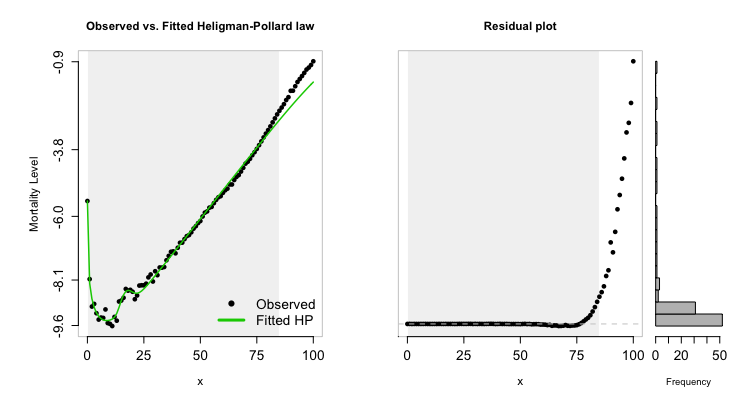
\includegraphics[scale=0.6]{Cap2/mortlaw02.png}
\captionsetup{width=1.1\linewidth}
\caption[Ajuste del modelo de Heligman-Pollard]{Ajuste del modelo de Heligman-Pollard para los datos de nivel de mortalidad de la población española}\\
\textit{(Fuente: Elaboración propia en \textbf{R} a partir de Human Mortality Database y Pascariu [2018])}
\end{figure}

\newpage
\begin{figure}[!htp]
\centering
%\hspace*{-1cm}
\vspace{-0.3cm}
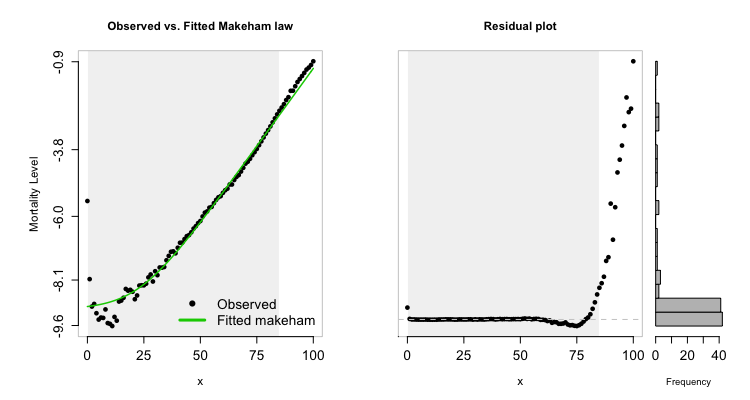
\includegraphics[scale=0.58]{Cap2/mortlaw03.png}

\vspace{-0.3cm}
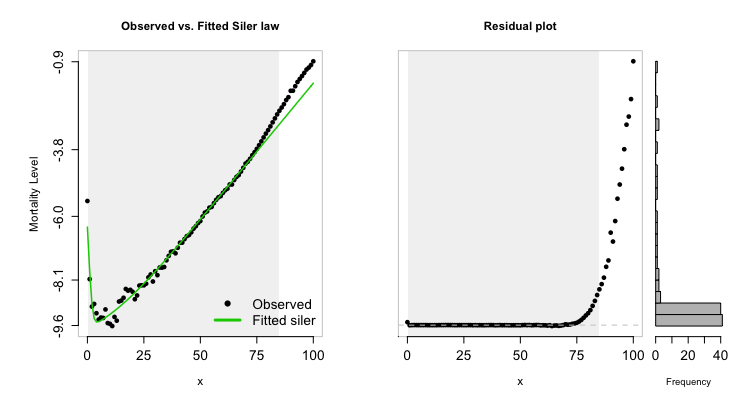
\includegraphics[scale=0.58]{Cap2/mortlaw04.png}

\vspace{-0.3cm}
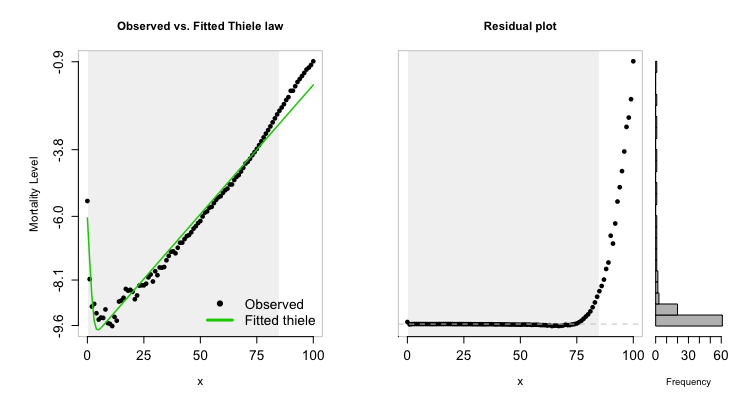
\includegraphics[scale=0.58]{Cap2/mortlaw05.png}
\captionsetup{width=1.1\linewidth}
\caption[Ajuste de los datos a los modelos de Makeham, Siler y Thiele]{Ajuste de los modelos de Makeham, Siler y Thiele para los datos de nivel de mortalidad de la población española}\\
\textit{(Fuente: Elaboración propia en \textbf{R} a partir de Human Mortality Database y Pascariu [2018])}
\end{figure}

Otro análisis y proyección interesante que hemos simulado ha sido el propuesto por Pascariu (2018) \textcolor{red}{[106]}, en el que afirma que la esperanza de vida está estrechamente correlacionada no solo entre países sino entre hombres y mujeres; así, construye un modelo que usa las correlaciones existentes entre países y entre sexos para proyectar la esperanza de vida de forma separada al nacer y a partir de los 65 años en el modelo denominado \textit{Double-Gap} (DG), comparándolo con los de Lee-Carter y Cairns-Blake-Dowd.\\

En base a lo anterior, para predecir los niveles futuros de esperanza de vida, el autor identifica el punto de referencia que dé la mejor predicción de la esperanza de vida (esto es, el mejor ajuste que den los modelos usados) para obtener un sentido general de la dirección y la tasa de cambio en la mortalidad humana. La brecha entre la esperanza de vida femenina en una población dada y la tendencia (según los mejores ajustes de los modelos disponibles), $D_{k,x,t}$, se pronostica utilizando un modelo clásico de series de tiempo, determinando así la esperanza de vida femenina futura. La brecha entre la esperanza de vida masculina y femenina, $G_{k,x,t}$ se pronostica con la ayuda de un modelo mixto para obtener la esperanza de vida masculina específica del país.

 $$\nabla^{d} D_{k, x, t}=\underbrace{\mu_{k, x}}_{\text { Drift }}+\underbrace{\sum_{i=1}^{p} \phi_{i} \nabla^{d} D_{k, x, t-i}}_{\text { Regresión }}+\underbrace{\epsilon_{k, x, t}^{(1)}+\sum_{j=1}^{q} \theta_{j} \epsilon_{k, x, t-j}^{(1)}}_{\text { Ruido suavizado }}$$

\[
    G_{k,x,t}^{*}= \begin{cases}
                  \beta_{0}+\underbrace{\beta_{1} G_{k, x, t-1}+\beta_{2} G_{k, x, t-2}}_{\text { Modelo autorregresivo }}+\underbrace{\beta_{3}(e_{k, x, t}^{f}-\tau)_{+}}_{\substack{\text {Nivel asociado a la esperanza de vida }\\ \text{cuando el gap empieza a estrecharse}}}+\epsilon_{k, x, t}^{(2)} \quad \text { si, }\hspace{0.3cm} e_{k, x, t}^{f} \leq A\\
                 \underbrace{G_{k, x, t-1}+\epsilon_{k, x, t}^{(3)}}_{\text { Proceso aleatorio }}\ \  \hspace{7cm} \text{en otro caso}
                \end{cases} 
  \]

Con el uso del paquete \textbf{`MortalityGap'} disponible en \textit{\textbf{R}}, hemos podido simular y adaptar este modelo para la población española donde en el periodo que va desde 1950 hasta 2014, (periodo de disponibilidad de cifras reales en la \textit{Human Mortality Database}, fuente de origen de los datos) el modelo que mejor se ajusta para describir los datos es el ARIMA(1, 0, 2) tanto para la edad 0, esto es al nacer como a los 65 años.\\

%\begin{table}[htp]
%\begin{center}
%\begin{tabular}{lllllll} \hline
 %      & \textit{Edad} & \textit{Rango}   & $\mu$ & $\phi_{1}$ & $\phi_{2}$ & $\theta_{1}$ \\ \hline
%\multirow{2}{*}{\textit{España}} & 0    & (1, 0, 2) &       &              &              &              \\
  %     & 65   & (1, 0, 2) &       &              &              & \\   \hline         
%\end{tabular}
%\captionsetup{width=0.46\linewidth}
%\caption[Parámetros estimados del modelo ARIMA]{Parámetros estimados del modelo ARIMA para el `gap' entre la mejor predicción y los datos de España al nacimiento y a la edad de 65 años, 1950–2014.}\\
%\textit{Fuente: Cálculos propios en \textbf{R} a partir de HMD y Pascariu [2018]}
%\end{center}
%\end{table}

%\vspace{-0.3cm}
Las estimaciones de los parámetros del modelo se proporcionan en el \textbf{cuadro 2.1} para los ajustes al nacer y a los 65 años, respectivamente. El coeficiente $\beta_{0}$ refleja el nivel de interceptación, el cual puede ser interpretado como la brecha biológica entre sexos; $\beta_{1}$ y $\beta{_2}$ representan el efecto de las dos brechas previos en $t-1$ y $t-2$, lo que influye en el rango de valores posibles para la nueva brecha. Juntos, los tres primeros parámetros, $\beta_{0}$, $\beta_{1}$ y $\beta_{2}$ explican la mayoría de la tendencia de la brecha. El parámetro negativo $\beta_{3}$ proporciona la velocidad de la convergencia entre la esperanza de vida femenina y masculina, por lo que como se puede ver, las esperanzas de vida al nacimiento convergen más rápido que aquéllas a la edad de 65 años.

%\newpage
\begin{table}[htp]
\begin{center}
\begin{tabular}{p{2cm}p{2.5cm}p{2.5cm}p{3cm}} \hline
\multirow{2}{*}{\textit{Parámetros}}  & \textit{Estimación} & \textit{Estimación} & $Pr(\textgreater |t|)$ \\ 
            & \textit{Edad 0}     & \textit{Edad 65}    & \textit{para ambas edades}    \\ \hline
$\beta_{0}$ &     0.2125737       & 0.1405291 &     < 2.2e-16                 \\ 
$\beta_{1}$ &   0.8218405       &    0.6480704         &    < 2.2e-16    \\
$\beta_{2}$ &  0.1597114          &    0.3294324        &        < 2.2e-16    \\
$\beta_{3}$ &   -0.0269039          &  -0.0144203           &       < 2.2e-16    \\
$\tau$  &  75             &      15      &                      \\
$A$   &  86               &      24      &                      \\
$L$   &  2.24               &       0.33     &                      \\ 
$U$    &  13.68               &       5.24     &                     \\ \hline
\end{tabular}
\captionsetup{width=1\linewidth}
\caption[Parámetros estimados para el `gap' entre la esperanza de vida al nacimiento y 65]{Parámetros estimados para el `gap' entre la esperanza de vida al nacimiento y a la edad de 65 años}\\
\textit{Fuente: Cálculos propios en \textbf{R} a partir de HMD y Pascariu [2018]}
\end{center}
\end{table}

\newpage
Los valores futuros estimados para el año 2050, gap incluido, junto a los intervalos de predicción al 80\% y 95\%, son mostrados en la \textbf{figura 2.16}. A partir del año 2014 se producen las proyecciones por sexo (modelo DG, línea discontinua en azul), siendo la parte de color claro azulado el `gap' (hueco) entre sexos.

\vspace{-0.3cm}
\begin{figure}[!htp]
\centering
\hspace*{-0.5cm}
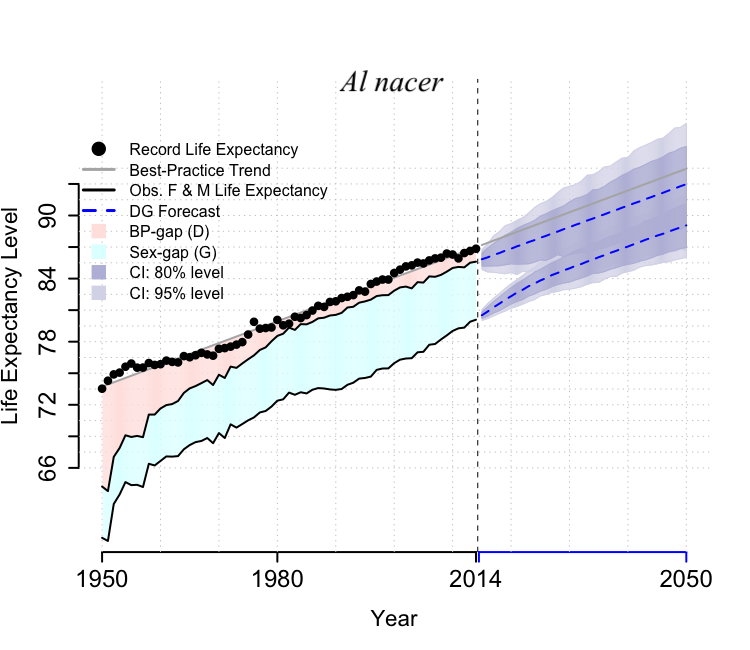
\includegraphics[scale=0.35]{Cap2/mortgap01.png}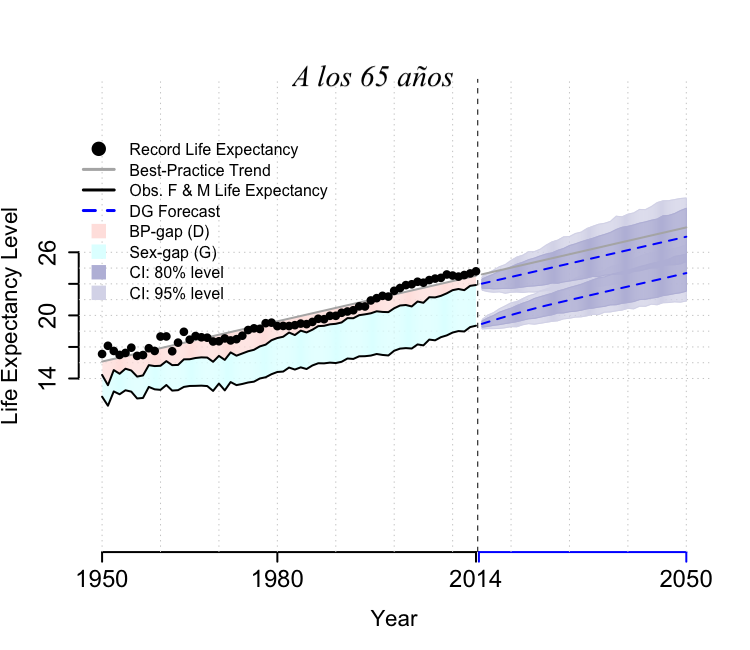
\includegraphics[scale=0.35]{Cap2/mortgap03.png}
\captionsetup{width=0.85\linewidth}
\caption[Esperanza de vida y proyectada con varios modelos]{Esperanza de vida actual y proyectada al nacer y a partir de los 65 años generada por los modelos Double-Gap (DG), Lee-Carter (LC) y Cairns-Blake-Dowd (CBD), para hombres y mujeres, 1950-2050. Los intervalos de predicción al 80\% y al 95\% solo se muestran para el modelo DG }\\
\textit{(Fuente: Elaboración propia en \textbf{R} a partir de Human Mortality Database y Pascariu [2018])}
\end{figure}

El \textbf{cuadro 2.2} muestra los resultados de la gráfica en conexión con los datos históricos, a partir de los cuales se hacen las proyecciones hasta el año 2050, observándose que según el modelo DG, la esperanza de vida femenina al nacer sería de 92.97 años y la masculina de 89.08, siendo la brecha de 3.89 años. A los 65 años, dicha esperanza de vida femenina sería de 27.73 años y la masculina de 24.29, con una reducción en la brecha, pasando ésta a 3.89 años.

\begin{table}[htp]
\begin{center}
\begin{tabular}{llllllllll}\hline
       & \multirow{2}{*}{Modelo} &              & \multicolumn{3}{c}{Edad 0}   &  & \multicolumn{3}{c}{Edad 65}        \\ \cline{4-6} \cline{8-10} 
       &        &              & \cellcolor[gray]{0.85}Mujer  & \cellcolor[gray]{0.85}Hombre & \cellcolor[gray]{0.85}Brecha &  & \cellcolor[gray]{0.85}Mujer   & \cellcolor[gray]{0.85}Hombre & \cellcolor[gray]{0.85}Brecha \\ \hline
España & DG     & $\hat{e}_{x,2050}$ & 92.97  & 89.08  & 3.89   &  & 27.73   & 24.29  & 3.43\\  \hline
\end{tabular}
\captionsetup{width=1\linewidth}
\caption[Proyecciones estimadas de la esperanza de vida año 2050 entre hombres y mujeres ]{Proyecciones de la esperanza de vida en hombres y mujeres incluyendo la brecha, al nacer y a los 65 años.}\\
\textit{Fuente: Cálculos propios en \textbf{R} a partir de HMD y Pascariu [2018]}
\end{center}
\end{table}

Finalmente, y como mencionamos al comienzo de este análisis, es interesante simular las proyecciones de esperanza de vida y mortalidad con uno de los modelos clásicos que siguen siendo más utilizados, el de de Lee-Carter. Para ello hemos seguido utilizando nuestros datos ya utilizados en nuestras anteriores simulaciones y los hemos ajustado al modelo (el código en \textsf{\textbf{R}} se encuentra disponible en el \textbf{anexo E}) $$\text{ln}\ m_{x,t}=a_{x}+b_{x}k_{t}+\epsilon_{x,t}$$ donde $a_{x}$ describe la forma general de mortalidad según las diferentes edades y representa el logaritmo de la media geométrica de las tasas de mortalidad empírica, promediada a lo largo de años históricos; $e^{a_{x}}$ mide de hecho la forma general a través de la edad del calendario de mortalidad. Además, $k_{t}$ reproduce la tendencia temporal subyacente, mientras que un término $b_{x}$ se considera para tener en cuenta el efecto diferente del tiempo $t$ en cada edad. Se supone que $b_{x}$ es invariante en el tiempo y explica cómo las tasas disminuyen rápida o lentamente en respuesta al cambio en $k_{t}$.\\
Finalmente $\epsilon_{x,t}$ son variables aleatorias \textit{N(0; 2)} independientes e idénticamente distribuidas, teniendo en cuenta que tanto la edad como la tendencia temporal no son capturadas en su totalidad por el modelo.\\

La (\textbf{figura 2.17}) muestra, para la población española, el patrón de logaritmo de las tasas de mortalidad según la edad y el tiempo. Se muestran varios comportamientos respectivamente para hombres, mujeres y población total.

\begin{figure}[!htp]
\centering
%\hspace*{-0.7cm}
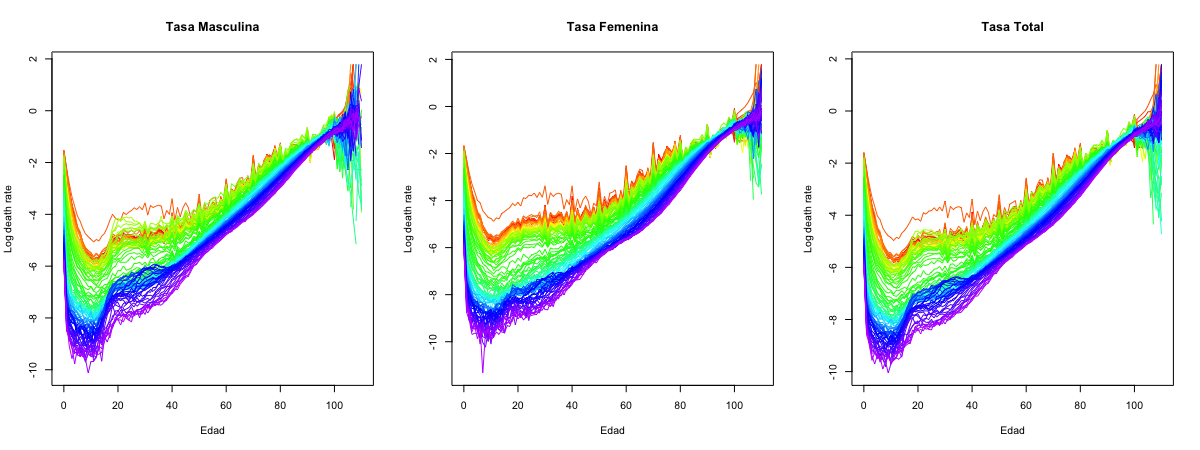
\includegraphics[scale=0.44]{Cap2/spain01.png}
\includegraphics[scale=0.44]{Cap2/spain02.png}
\captionsetup{width=1\linewidth}
\caption{Patrón de logaritmo de tasas de mortalidad según edad y tiempo para la población española}
\textit{Fuente: Cálculos propios en \textbf{R} a partir de HMD}\end{figure}
\end{figure}

Los datos españoles confirman que la mortalidad disminuye en todas las edades con un comportamiento diferente según los diferentes años de vida.\\

Para ajustar el modelo Lee - Carter (sin el cambio logarítmico) se puede usar la función en \textit{\textbf{R}} \texttt{`lca'}. Lee-Carter se aplica aquí por separado entre hombres, mujeres y población total y al considerar una edad máxima igual a 100. De esta forma, adaptando el código \textit{\textbf{R}} como sigue:\\

{
\setlength{\fboxsep}{0.75pt}%
\noindent\setlength{\fboxrule}{0pt}%
\fbox{%
{\colorbox{gray!20}{\parbox{1\linewidth}{%
\small{\texttt{>\ spainLcaM<-lca(spainDemo,series="male",max.age=100)\\
>\ spainLcaF<-lca(spainDemo,series="female",max.age=100)\\
>\ spainLcaT<-lca(spainDemo,series="total",max.age=100)
}}}}}}}\\

dicha función devuelve el objeto que nos permite inspeccionar $a_{x}, b_{x}$ y $k_{t}$. La \textbf{figura 2.18} representa los valores de los parámetros estimados:

\newpage
\begin{figure}[!htp]
\centering
\hspace*{-0.7cm}
\includegraphics[scale=0.44]{Cap2/spain03.png}
\caption{Parámetros $a_{x}, b_{x}, k_{t}$ estimados con la función \texttt{`lca'}}
\textit{Fuente: Cálculos propios en \textbf{R} a partir de HMD}
\end{figure}

Un comportamiento similar de los parámetros se observa de acuerdo con diferentes conjuntos de datos. Como se esperaba, la mortalidad promedio crece cuando aumenta la edad (ver patrón de $\hat{a}_{x}$). $b_{x}$ muestra, en cambio, un mayor valor para las edades más jóvenes y una mayor mejora para las mujeres en el rango de edad (60-80). Finalmente, como se esperaba, $k_{t}$ tiene una tendencia decreciente con el incremento de tiempo.\\

A continuación podemos usar la función \texttt{`forecast'} para predecir $k_{t}s$ (hasta 110 años). La proyección está basada en una extrapolación ARIMA (\textbf{figura 2.19})\\

{
\setlength{\fboxsep}{0.75pt}%
\noindent\setlength{\fboxrule}{0pt}%
\fbox{%
{\colorbox{gray!20}{\parbox{1\linewidth}{%
\small{\texttt{>\ fM <- forecast(spainLcaM, h = 110)\\
>\ fF <- forecast(spainLcaF, h = 110)\\
>\ fT <- forecast(spainLcaT, h = 110)
}}}}}}}\\

\begin{figure}[!htp]
\centering
\hspace*{-1cm}
\includegraphics[scale=0.38]{Cap2/spain04.png}
\caption{Valores pronosticados de $k_{t}$ re-escalados a cero en el último año observado (2014)}
\textit{Fuente: Cálculos propios en \textbf{R} a partir de HMD}
\end{figure}

Finalmente, derivamos el patrón completo de las tasas, las cuales, pasadas y pronosticadas se unen aquí en la misma matriz (ver \textbf{figura 2.20}).\\

{
\setlength{\fboxsep}{0.75pt}%
\noindent\setlength{\fboxrule}{0pt}%
\fbox{%
{\colorbox{gray!20}{\parbox{1\linewidth}{%
\small{\texttt{>\  ratesM<-cbind(spainDemo\$rate\$male[1:100,],fM\$rate\$male[1:100,])\\
>\  ratesF<-cbind(spainDemo\$rate\$female[1:100,],fF\$rate\$female[1:100,])\\
>\  ratesT<-cbind(spainDemo\$rate\$total[1:100,],fT\$rate\$total[1:100,])
}}}}}}}\\

\newpage
Presentamos aquí el patrón de tasas pasadas y pronosticadas según la diferente población. La mejora prevista esperada es claramente visible:

\begin{figure}[!htp]
\centering
\includegraphics[scale=0.45]{Cap2/spain05.png}
\captionsetup{width=1.1\linewidth}
\caption{Tasas de observación y predicción de fallecimiento para la población}
\end{figure}

En el paquete \textbf{`StMoMo'}, la rutina de arranque de los modelos de mortalidad estocástica GAPC se implementa con la función genérica \texttt{bootstrap}. Esta función es compatible tanto con el \textit{bootstrap} semiparamétrico como con el \textit{bootstrap} residual. Por ejemplo, nosostros hemos obtenido 5 000 muestras de arranque semiparamétricas del modelo Lee-Carter con la función:\\

{
\setlength{\fboxsep}{0.75pt}%
\noindent\setlength{\fboxrule}{0pt}%
\fbox{%
{\colorbox{gray!20}{\parbox{1\linewidth}{%
\small{\texttt{
>\  LCboot\_NZ <- bootstrap(LCfit\_NZ, nBoot = 5000, type = "semiparametric")
}}}}}}}\\

El bootstrap es un procedimiento de computación intensiva. En particular, las 5 000 muestras semiparamétricas de arranque del modelo de Lee-Carter tardaron aproximadamente dos horas en ejecutarse.\\

La salida de la función  \texttt{bootstrap} es un objeto de la clase \texttt{``bootStMoMo''} en el que el componente \texttt{bootParameters} contiene las réplicas \texttt{nBoot} de los parámetros de bootstrap. Con el comando se puede obtener un gráfico de abanico que muestra los intervalos de confianza del 50\%, 80\% y 95\% del modelo de arranque y carga de Lee-Carter \textbf{(figura 2.21)}:

\vspace{-0.3cm}
\begin{figure}[!htp]
\centering
\hspace*{-0.5cm}
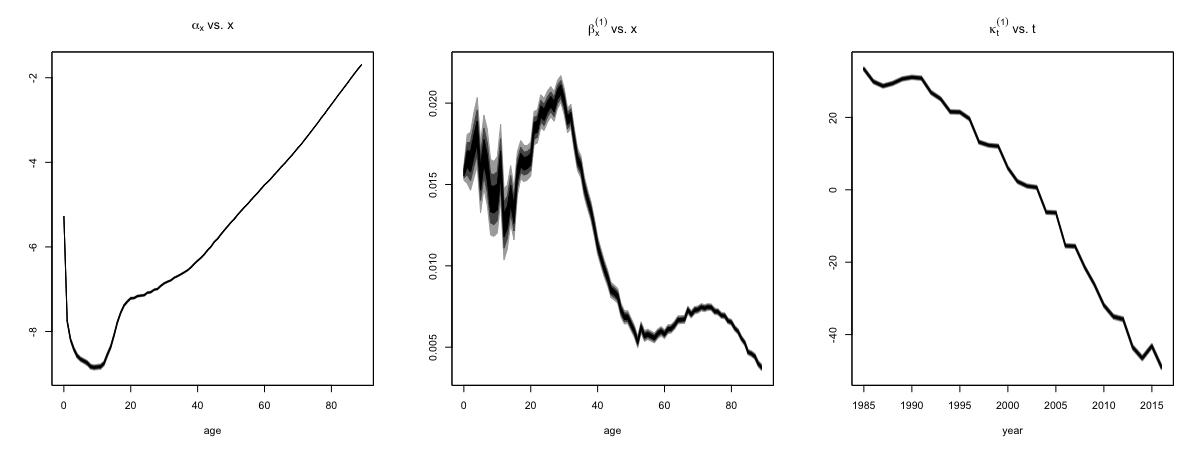
\includegraphics[scale=0.43]{Cap2/stmomo01.png}
\captionsetup{width=1\linewidth}
\caption[Parámetros obtenidos con la técnica \textit{bootstrap} para el modelo de Poisson Lee-Carter]{Parámetros obtenidos con la técnica \textit{bootstrap} para el modelo de Poisson Lee-Carter se ajustaron a la población masculina de España para las edades 0-89 y el período 1985-2016. Las sombras en el abanico representan intervalos de confianza al 50\%, 80\% y 95\%.}
\end{figure}

Se puede apreciar que mientras la incertidumbre de los parámetros en la función de edad estática $\alpha_{x}$ y el índice de período $k_{t}^{(1)}$ es modesta, la incertidumbre en los parámetros de modulación de la edad $\beta_{t}^{(1)}$ es más significativa.\\

Para resaltar el impacto del riesgo de parámetros en las proyecciones de la tasa de mortalidad, es interesante comparar los intervalos de predicción con y sin el margen de incertidumbre de los parámetros. Con 24 años de anticipación, el pronóstico central junto con las 5 000 trayectorias del modelo Lee-Carter permite solo un error de pronóstico en el proceso aleatorio con deriva e ignorando el error de ajuste del modelo se puede obtener con el código:\\

{
\setlength{\fboxsep}{0.75pt}%
\noindent\setlength{\fboxrule}{0pt}%
\fbox{%
{\colorbox{gray!20}{\parbox{1\linewidth}{%
\small{\texttt{>\  LCsimPU\_ESP <- simulate(LCboot\_ESP,  h = 24)\\
>\  LCfor\_ESP <- forecast(LCfit\_ESP, h = 24)\\
>\  LCsim\_ESP <- simulate(LCfit\_ESP, nsim = 5000, h = 24)
}}}}}}}\\

La \textbf{figura 2.22} muestra los intervalos de predicción del 95\% para las tasas de mortalidad a los 40, 60 y 80 años, con y sin margen para la incertidumbre de los parámetros.

\vspace{-0.3cm}
\begin{figure}[!htp]
\centering
%\hspace*{-0.5cm}
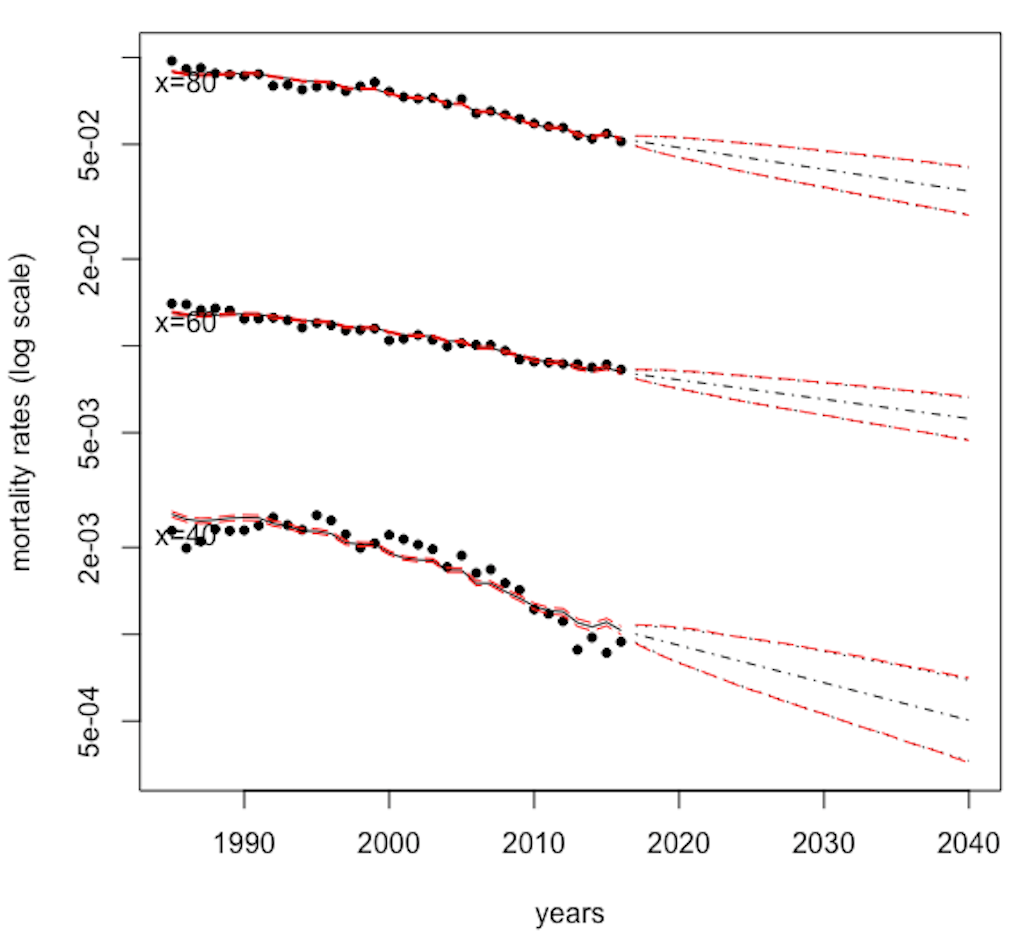
\includegraphics[scale=0.45]{Cap2/stmomo02.png}
\captionsetup{width=1\linewidth}
\caption[Intervalos de predicci\'on para las tasas de mortalidad]{Intervalos de predicci\'on al 95\% para tasas de mortalidad $q_{xt}$ para las edades $x=40$ (l\'ineas inferiores), $x=60$ (l\'ineas del medio) y $x=80$ (l\'ineas superiores) para el modelo Poisson Lee-Carter, ajustado al total de la poblaci\'on espa\~nola para el intervalo de edad 0-90 y el periodo correspondiente 1985-2014. La l\'inea de puntos muestran las tasas hist\'oricas de mortalidad entre 1985 y 2014 y las l\'ineas s\'olidas negras muestran las correspondientes tasas ajustadas. Las l\'ineas discont\'inuas representan el pron\'ostico central, las l\'ineas punteadas en negro representan los intervalos de predicci\'on al 95\% excluyendo el par\'ametro incertidumbre y las l\'ineas discont\'inuas punteadas en rojo representan los intervalos de confianza y predicci\'on al 95\% incluyendo el par\'ametro incertidumbre.}
\end{figure}

Se puede ver claramente que la incertidumbre de los parámetros tiene un impacto importante en los intervalos de predicción. Esto es particularmente notable a la edad de 40 años, donde en el año 2030, por ejemplo, el ancho del intervalo de predicción con la incertidumbre del parámetro es aproximadamente 3 veces mayor que el de la incertidumbre del parámetro.

%\begin{figure}[!htp]
%\centering
%\hspace*{-1cm}
%\includegraphics[scale=0.44]{Cap2/LC00.png}
%\end{figure}

%\begin{figure}[!htp]
%\centering
%\hspace*{-1cm}
%\includegraphics[scale=0.4]{Cap2/LC01.png}
%\hspace*{-1cm}
%\includegraphics[scale=0.44]{Cap2/LC02.png}
%\end{figure}

%\begin{figure}[!htp]
%\centering
%\includegraphics[scale=0.44]{Cap2/LC03.png}
%\end{figure}

%----------------------------------------------------------------------------------------
%\newpage
\section{Conclusiones del capítulo}

Las predicciones sobre los fenómenos demográficos han ido ganando importancia en las últimas décadas a medida que la esperanza de vida ha ido aumentando con rapidez. A lo largo de todos estos años se han propuesto una gran cantidad de enfoques diferentes para modelar estos fenómenos que van desde los más simples (el programa modelo de la ONU) hasta los más complicados (el modelo Coale-Trussell, por ejemplo). Aquí hemos hecho una revisión de la literatura que ha tratado de recoger aquellos que, de alguna forma u otra, han contribuido al avance de esta materia y hemos comprobado el funcionamiento de algunos de ellos ajustándolos y adaptándolos a nuestras necesidades y datos de la población española, con resultados en la línea de lo revisado en la teoría.\\

Es importante destacar que la precisión de los modelos de predicción de los fenómenos demográficos es un indicador importante al juzgar la calidad de los pronósticos de la población. En aspectos como el contenido de la información, por ejemplo, cabría preguntarse si el pronóstico predice solo la población total o también los grupos de edad. En fines políticos, por otro lado, es relevante discernir si la tendencia prevista implica medidas políticas inmediatas. Sin embargo, el grado en que el pronóstico refleja las tendencias reales es un factor clave para evaluar su calidad, en particular cuando el pronóstico se utiliza para fines de planificación. Por ejemplo, imaginemos un pronóstico para el cual las probabilidades son una contra dos que cubrirán las tendencias reales. Este pronóstico debe manejarse mucho más cautelosamente que uno que puede esperarse que sea erróneo solo una de cada cinco veces.\\

Los estudios han demostrado que un modelo de tres parámetros puede capturar la mayor parte de la variación en los esquemas de fertilidad y mortalidad observados. Los modelos con más parámetros, para la mayoría de los propósitos, no son necesarios, y pueden experimentarse dificultades para adaptar dichos modelos a un pequeño número de datos, como hemos visto en la parte de la revisión de la literatura, donde hacíamos referencia al trabajo de Wang y otros (2018) [86].\\

Los modelos que hemos utilizado, adaptado a la población española y usado para simular proyecciones a decenas de años vista, son una herramienta muy útil para medir y manejar el riesgo de longevidad. Este es un problema importante para aquellos que desean cubrir dicho riesgo utilizando índices de mortalidad publicados, ya sean gobiernos, planes de pensiones, aseguradoras o bancos. Además, el riesgo basado en la longevidad, a la vez que un desafío no solo para demógrafos, estadísticos, actuarios, sino también para organismos oficiales, también puede presentar un problema más amplio para las compañías de seguros que utilizan, en sus modelos de reserva, datos externos, como datos de población, en lugar de sus propios datos de política interna. La necesidad de cuantificar y reservar para cualquier riesgo de base potencial está recibiendo un enfoque cada vez mayor, particularmente bajo Solvencia II, por lo tanto y en vista de los continuos aumentos en la esperanza de vida, el uso de mejores métodos disponibles es ahora obligatorio, en particular por parte de los actuarios que practican en la industria de seguros y riesgos financieros, donde las ramificaciones de los pronósticos inexactos son agudas y aunque las magnitudes del envejecimiento son inciertas, y los errores de pronóstico probablemente son grandes, las políticas de envejecimiento pueden anticiparse a esto, la incertidumbre no debe implicar inacción y los pronósticos contienen información que se pueden usar en el diseño de políticas sociales que tendrán un impacto tanto en la población presente como, sobre todo, en la futura.

%Accuracy statistics of the type given here are important indicators when judging the quality of population forecasts. Other aspects, such as the information content (for instance, does the forecast predict only total population, or also age groups?) and the usefulness for policy purposes (for instance, does the predicted trend imply immediate policy measures?) are relevant as well. Nevertheless, the degree to which the forecast reflects real trends is a key factor in assessing its quality, in particular when the forecast is used for planning purposes. For example, imagine a forecast, for which the odds are one against two that it will cover actual trends. This forecast should be handled much more cautiously than one that can be expected to be in error only one out of five times.

%Fertility models find use in a wide variety of situations, for example, to smooth observed data as inputs into population projections, or other analytical exercises.

%A large number of different approaches to modelling fertility have been proposed over the years, ranging from the very simple (the UN model schedule), to the rather complicated (the Coale-Trussell model).

%Studies have shown that a three-parameter model can capture most of the variation in observed fertility schedules. Models with more parameters are, for most purposes, not required, and difficulties may be experienced in fitting such models to a small number of data points.

%The relational Gompertz model is a highly flexible three-parameter system for modelling fertility, which has found application in many areas of demographic work.

%----------------------------------------------------------------------------------------

\newpage

\section*{Referencias bibliogr\'aficas}
\addcontentsline{toc}{section}{\protect\numberline{}Referencias bibliogr\'aficas}%

\noindent \textcolor{red}{[1]} Siegel, J. S. y Swanson, D. A. (Editores): \textbf{``The Methods and Materials of Demography''}, Elsevier Academic Press, (2004).\\

\noindent \textcolor{red}{[2]} Sevcíková, H., Alkema, L. y Raftery, A. E.: \textbf{``bayesTFR: An R Package for Probabilistic Projections of the Total Fertility Rate''}, \textit{Journal of Statistical Software}, vol. 43, (1), (julio, 2011).\\ 

\noindent \textcolor{red}{[3]} Lee, R. D. y Carter, L. R.: \textbf{``Modeling and Forecasting U. S. Mortality}, \textit{Journal of the American Statistical Association''}, n\textsuperscript{o} 87 (419), p\'ags. 659-671, (1992).\\

\noindent \textcolor{red}{[4]} Cairns, A. J. G., Blake, D., Dowd, K., Coughlan, G.D., Epstein, D., y Khalaf-Allah, M.: \textbf{``Mortality Density Forecasts: An Analysis of Six Stochastic Mortality Models''}, \textit{Insurance: Mathematics and Economics}, n\textsuperscript{o}48 (3), p\'ags.: 355–367, (2011).\\

\noindent \textcolor{red}{[5]} Villegas, A. M., Millossovich, P. y Kaishev, V.: \textbf{``StMoMo: An R Package for Stochastic Mortality Modelling''}, R package version 0.4.0, \textsc{url:} \texttt{http://CRAN.R-project.org/package=StMoMo}, (2017). \\

\noindent \textcolor{red}{[6]} Hyndman, R.J., Booth, H., Tickle, L. y Maindonald, J.: \textbf{``Demography: Forecasting Mortality, Fertility, Migration and Population Data''}. R package version 1.18, \textsc{url:}  \texttt{http://CRAN.R-project.org/
package=demography}, (2014).\\

\noindent \textcolor{red}{[7]} Vinuesa, E. y otros: \textbf{``Demografía: Análisis y Proyecciones''}, Ed. Síntesis, (1997).\\

\noindent \textcolor{red}{[8]} Hoem, J. M., Madsen, D., Nielsen, J. L., Ohlsen, E., Hansen, H. O. y Rennermalm, B.: \textbf{``Experiments in Modelling Recent Danish Fertility Curves''}, \textit{Demography}, 18: 231-244, (1981).\\ 

\noindent \textcolor{red}{[9]} Davis, K. y Blake, J.: \textbf{`` Social Structure and Fertility: An Analytic Framework}, \textit{Economic Development and Cultural Change} 4 (3), págs.: 211–235, (1956).\\

\noindent \textcolor{red}{[10]} Bongaarts, J. y Potter, R.: \textbf{``Fertility, Biology, and Behavior: An Analysis of the Proximate Determinants''} New York: Academic Press, (1983).\\

\noindent \textcolor{red}{[11]} Aguinaga Roustan, J.: \textbf{``Bongaarts: Un Modelo de Fecundidad y su Aplicación en España''} \textit{Boletín de la Asociación de Demografía Histórica}, XIII, 3, págs.: 79-94, (1995).\\

\noindent \textcolor{red}{[12]} Del Pino Artacho, J. A.: \textbf{``Integración de Modelos en la Explicación de la Fecundidad''}, \textit{Cuadernos Geográficos}, 36, págs.: 105-124, (2005).\\

\noindent \textcolor{red}{[13]} Peristera, P. y Kostaki, A.: \textbf{``Modeling Fertility in Modern Populations''}, \textit{Demographic Research}, Vol. 16, art. 6, págs.: 141-194, (2007).\\

\noindent \textcolor{red}{[14]} Coleman, D. A.: \textbf{“New Patterns and Trends in European Fertility: International and Subnational Comparisons”}, en D. A. Coleman (Ed.), \textit{Europe's Population in the 1990s}, Oxford University Press, p\'ags.: 1-61, (1996).\\

\noindent \textcolor{red}{[15]} Sigle-Rushton, W.: \textbf{``England and Wales: Stable Fertility and Pronounced Social Status Differences''}, \textit{Demographic Research}, vol. 19, págs.: 455-502, (julio, 2008).\\

\noindent \textcolor{red}{[16]} Bray, H.: \textbf{``2006-Based National Population Projections For The UK and Constituent Countries''}, \textit{Population Trends}, n\textsuperscript{o}100, págs.: 32-39, (2008).\\

\noindent \textcolor{red}{[17]} Chandola. T., Coleman, D. A. y Horns, R. W.: \textbf{``Recent European Fertility Patterns: Fitting Curves to `distorted' distributions}, \textit{Population Studies}, 53, 3: 317-329, (1999).\\

\noindent \textcolor{red}{[18]} Hadwiger, H.: \textbf{“Una Función de Reproducción Analítica para Entidades Biológicas”}, \textit{Skandinavisk Aktuareitidskrift}, vol. 23, págs.: 101-113, (1940).\\

\noindent \textcolor{red}{[19]} Coale, A.J. y Trussell, T. J.: \textbf{``Model Fertility Schedules: Variations in the Age Structure of Childbearing in Human Populations''}, \textit{Population Index}, 40, 2, págs.:185-258, (1974).\\

\noindent \textcolor{red}{[20]} Coale, A.J. y Trussell, T. J.:  \textbf{``Technical Note: Finding the Two Parameters that Specify a Model Schedule of Marital Fertility''}, \textit{Population Index}, 44, 2, págs.: 203-214, (1978).\\

\noindent \textcolor{red}{[21]} Xie, Y.: \textbf{``What is Natural Fertility? The Remodelling of a Concept''}, \textit{Population Index}, 56, págs.: 656-663, (1990).\\

\noindent \textcolor{red}{[22]} Xie, Y. y Pimentel, Ellen E.: \textbf{``Age Patterns of Marital Fertility: Revising the Coale-Trussell Method''}, \textit{Journal of the American Statistical Association}, Vol. 87, No. 420, págs.: 997-984, (Diciembre, 1992).\\

\noindent \textcolor{red}{[23]} Hoem, J. M. y Rennermalm, B.: \textbf{``On the Statistical Theory of Graduation by Splines''}, \textit{University of Copenhagen}, Laboratory of Actuarial Mathematics. Working Paper No. 14, (1978).\\

\noindent \textcolor{red}{[24]} Gilks, W. R.: \textbf{``The Relationship Between Birth History and Current Fertility in Developing Countries''}, \textit{Population Studies}, 40, (1986).\\

\noindent \textcolor{red}{[25]} Mitra, S.: \textbf{“The Pattern of Age-Specific Fertility Rates”}, \textit{Demography}, 4, págs.: 894-906, (1967).\\

\noindent \textcolor{red}{[26]} Nurul Islam, M. y Mallick, S.A.: \textbf{``On The Use of a Truncated Pearsonian Type III Curve in Fertility Estimation''}, \textit{Dhaka University Studies Part B Science} 35 (1): págs.: 23-32, (1987).\\

\noindent \textcolor{red}{[27]} Romaniuk, A.: \textbf{“A Three Parameter Model for Birth Projections”}, \textit{Population Studies}, 27, 3, págs.: 467-478, (1973).\\

\noindent \textcolor{red}{[28]} Brass, W.: \textbf{``The Graduation of Fertility Distributions by Polynomial Functions”}, \textit{Population Studies}, 14: págs.: 148-162, (1960).\\

\noindent \textcolor{red}{[29]} Brass, W.: \textbf{``Perspectives in Population Prediction: Illustrated by the Statistics of England and Wales (with discussion)”}, \textit{Journal of the Royal Statistical Society A}, 137: págs.: 532-583, (1974).\\

\noindent \textcolor{red}{[30]} Brass, W.: \textbf{``Population Projections for Planning and Policy''}. \textit{Papers of the East- West Population Institute}, No 55. Honolulu, Hawaii, (1978).\\ 

\noindent \textcolor{red}{[31]} Billari, F. C. y Kohler, H-P. : \textbf{``Patterns of Lowest-Low Fertility in Europe''}. \textit{Population Studies}, 58: 161-176, (2002).\\ 

\noindent \textcolor{red}{[32]} DellaPergola, S.: \textbf{``Population Trends and Scenarios in Israel and Palestine''}, Editores: Kacowicz y Lutomski, en \textit{Population Resettlement in International Conflicts: A Comparative Study}, New York, Rowman and Littlefield, págs.: 183-207, (2007).\\ 

\noindent \textcolor{red}{[33]} Cai, Y.: \textbf{``Assessing Fertility Levels in China Using Variable-\textit{r} Method''}, \textit{Demography}, 45:371-381, (2008).\\

\noindent \textcolor{red}{[34]} Hyndman, R. y Booth, H.: \textbf{``Stochastic Population Forecasting Using Functional Data Models for Mortality, Fertility and Migration''}, \textit{International Journal of Forecasting}, 24, págs: 323-342, (2008). \\

\noindent \textcolor{red}{[35]} Booth, H., Pennec, S. y Hyndman, R.: \textbf{``Stochastic Population Forecasting Using Functional Data Methods: The Case of France''}, \textit{Presented at the Annual Meeting of the International Union for the Scientific Study of Population, Marrakech; Morocco}, (Sep. 2009). \\

\noindent \textcolor{red}{[36]} Caltabiano, M., Castiglioni, M., Rossina, A.: \textbf{``Lowest-low Fertility: Signs of a Recovery in Italy?''}, \textit{Demographic Research}, 21:681-679, (2009).\\

\noindent \textcolor{red}{[37]} De Iaco, S. y Maggio, S.: \textbf{``A Dynamic Model for Age-specific Fertility Rates in Italy''}, \textit{Spatial Statistics}, (2015). \\

\noindent \textcolor{red}{[38]} V\"ahi, M.: \textbf{``Fertility Modelling''}. \textit{Papers on Anthropology}, XXVI/1, págs.: 107-114, (2017).\\

\noindent \textcolor{red}{[39]} Adsera, A.: \textbf{``Marital Fertility and Religion: Recent Changes in Spain''}, \textit{IZA Discussion Papers}, n\textsuperscript{o} 1399, (2004).\\

\noindent \textcolor{red}{[40]} Bermúdez, S., Blanquero, R., Hernández, J. A. y Planelles, J.: \textbf{``A New Parametric Model for Fitting Fertility Curves''}, \textit{Population Studies}, vol. 66, n\textsuperscript{o} 3, págs.:297-310, (november, 2018).\\

\noindent \textcolor{red}{[41]} Os\'es-Arranz, A. y Quilis, E. M.: \textbf{``Introducing Uncertainty on Fertility and Survival in the Spanish Population Projections: A Monte Carlo Approach''}, \textit{AIReF Working Paper DT/2018/5}, (2018).\\

\noindent \textcolor{red}{[42]} Alkema, L., Raftery, A. y otros: \textbf{``Probabilistic Projections of the Total Fertility Rate for All Countries''}, \textit{Demography}, 48 (3), págs.: 815-839, (agosto, 2011).\\ 

\noindent \textcolor{red}{[43]} United Nations, Department of Economic and Social Affairs, Population Division: \textbf{``World Population Prospects. The 2017 Revision''}, (2017). Disponible en {\texttt{\small{https://esa.un.org/unpd/wpp/publications/\\
files/wpp2017\_keyfindings.pdf}}}\\

\noindent \textcolor{red}{[44]} Lindley, D.V. y Smith, A.F.M.: \textbf{``Bayes Estimates for the Linear Model''}, \textit{Journal of the Royal Statistical Society B}, 34, págs.: 1-41, (1972).\\ 

\noindent \textcolor{red}{[45]} Gelman, A., Carlin, J.B., Stern, H.S. y Rubin, D.B.: \textbf{``Bayesian Data Analysis''}, 2\textsuperscript{a} edición. Chapman \&Hall/CRC, Boca Raton, Florida (2004).\\ 

\noindent \textcolor{red}{[46]} South, A.: \textbf{``rworldmap: For Mapping Global Data''}. \textsf{\textbf{R}} package version 0.1211. Disponible en:\\
{\texttt{\small{http://CRAN.R-project.org/package=rworldmap}}}.\\ 

\noindent \textcolor{red}{[47]} Furrer, R., Nychka, D. y Sain, S.: \textbf{``fields: Tools for Spatial Data''}. \textsf{\textbf{R}} package version 6.5.2. Disponible en: {\texttt{\small{http://CRAN.R-project.org/package=fields}}}.\\ 

\noindent \textcolor{red}{[48]} Gompertz, B.: \textbf{``On the Nature of the Function Expressive of the Law of Human Mortality, and on a New Mode of Determining the Value of Life Contingencies''}, \textit{Philosophical Transactions of the Royal Society of London}, vol. 115, págs.: 513-583, (1825).\\

\noindent \textcolor{red}{[49]} World Bank: \textbf{``Averting the Old Age Crisis: Policies to Protect the Old and Promote the Growth''}, \textit{World Bank Policy Research Report}, Oxford University Press, (1994).\\

\noindent \textcolor{red}{[50]} Alho, J. M.: \textbf{``Stochastic Methods in Population Forecasting''}, \textit{International Journal of Forecasting}, 6, págs. 521-530, (1990).\\

\noindent \textcolor{red}{[51]} Alho, J. M. y Spencer, B. D.: \textbf{``Statistical Demography and Forecasting''}, Ed. Springer, Nueva York, (2005).\\

\noindent \textcolor{red}{[52]} Tabeau, E.: \textbf{``A Review Of Demographic Forecasting Models For Mortality''}. En: E. Tabeau, A. Van Den Berg Jeths y C. Heathcote, editores: \textit{Forecasting Mortality in Developed Countries: Insights from a Statistical, Demographic and Epidemiological Perspective}, (1-32), Kluwer Academic Publishers, Dordrecht, (2001).\\

\noindent \textcolor{red}{[53]} Lee, R. D. y Carter, L. R.: \textbf{``Modeling and Forecasting U.S. Mortality''}, \textit{Journal of American Statistical Association}, vol. 87, n\textsuperscript{o} 419, págs. 659-671, (1992).\\

\noindent \textcolor{red}{[54]} Wilmoth, J. R.:  \textbf{``Computational Methods for Fitting and Extrapolating the Lee-Carter Model for Mortality Change''}, (Technical Report). Department of Demography, University of California, Berkeley, (1993).\\

\noindent \textcolor{red}{[55]} Lee, R. D.: \textbf{``The Lee-Carter Method for Forecasting Mortality with Various Extensions and Applications''}, \textit{North American Actuarial Journal}, 4 (1), págs. 80-93, (2000).\\

\noindent \textcolor{red}{[56]} Booth, H., Maindonald, J. y Smith, L.: \textbf{``Applying Lee-Carter Under Conditions of Variable Mortality Decline''}, \textit{Population Studies}, 56 (3), págs.: 325–36, (2002).\\

\noindent \textcolor{red}{[57]} Renshaw, A. y Haberman, S.: \textbf{``Lee-Carter Mortality Forecasting With Age-Specific Enhancement''}, \textit{Insurance: Mathematics and Economics}, 33 (2), págs.: 255–272, (2003).\\

\noindent \textcolor{red}{[58]} Hyndman, R. y Ullah, M.: \textbf{``Robust Forecasting of Mortality and Fertility Rates: A Functional Data Approach''}, \textit{Computational Statistics \& Data Analysis}, 51 (10), págs.: 4942–4956, (2007).\\

\noindent \textcolor{red}{[59]} Hatzopoulos, P. y Haberman, S.: \textbf{``A Parameterized Approach to Modeling and Forecasting Mortality''}, \textit{Insurance: Mathematics and Economics}, 44 (1), págs.: 103–123, (2009).\\

\noindent \textcolor{red}{[60]} Wang, J. L., Huang, H., Yang, S. S. y Tsai, J. T.: \textbf{ ``An Optimal Product Mix for Hedging Longevity Risk in Life Insurance Companies: The Immunization Theory Approach''}, \textit{Journal of Risk and Insurance}, 77 (2), 473–497.\\

\noindent \textcolor{red}{[61]} Cairns, A. J. G., Blake, D. y Dowd, K.: \textbf{``A Two-Factor Model For Stochastic Mortality with Parameter Uncertainty: Theory and Calibration''}, Journal of Risk and Insurance, 73 (4), 687–718, (2006).\\

\noindent \textcolor{red}{[62]} Cairns, A. J. G., Blake, D., Dowd, K., Coughlan, G. D., Epstein, D., Ong, A. y Balevich, I.: \textbf{``A Quantitative Comparison of Stochastic Mortality Models Using Data from England and Wales and the United States''}, \textit{North American Actuarial Journal}, 13 (1), 1–35, (2009).\\

\noindent \textcolor{red}{[63]} Glenn, N.: \textbf{``Cohort Analysts’ Futile Quest: Statistical Attempts to Separate Age, Period and Cohort Effects''}, \textit{American Sociological Review}, 41 (5), págs.: 900–904, (1976).\\

\noindent \textcolor{red}{[64]} Fienberg, S. E. y Mason, W. M.: \textbf{``Identification and Estimation of Age Period-Cohort Models in the Analysis of Discrete Archival Data''}, \textit{Sociological Methodology}, 10, 1–67, (1979).\\

\noindent \textcolor{red}{[65]} Rodgers, W.: \textbf{``Estimable Functions of Age, Period and Cohort Effects''}, \textit{American Sociological Review}, 47 (6), págs.: 774–787, (1982).\\

\noindent \textcolor{red}{[66]} Holford, T. R.: \textbf{``The Estimation of Age, Period and Cohort Effects for Vital Rates''}, \textit{Biometrics}, 39 (2), págs.: 311–324, (1983).\\

\noindent \textcolor{red}{[67]} Wilmoth, J. R.: \textbf{``Variation in Vital Rates by Age, Period and Cohort}. \textit{Sociological Methodology}, 20, págs.: 295–335, (1990).\\

\noindent \textcolor{red}{[68]} Kuang, D., Nielsen, B. y Nielsen, J. P.: \textbf{``Forecasting with the Age-Period-Cohort Model and the Extended Chain-Ladder Model''}, Biometrika 95 (4), págs.: 987–991, (2008).\\

\noindent \textcolor{red}{[69]} O’Brien, R. M.: \textbf{Constrained Estimators and Age-Period-Cohort models}. \textit{Sociological Methods \& Research}, 40 (3), págs.: 419–452, (2011).\\

\noindent \textcolor{red}{[70]} Currie, I. D.: \textbf{``On Fitting Generalized Linear and Non-Linear Models of Mortality''}, \textit{Scandinavian Actuarial Journal}, 4, 356-383, (2016).\\

\noindent \textcolor{red}{[71]} Hunt, A. y Blake, D.: \textbf{``On the Structure and Classification of Mortality Models''}, \textit{Pension Institute}, Discussion Paper PI-1506, (August, 2015), {\texttt{\small{http://www.pensions-institute.org}}}.\\

\noindent \textcolor{red}{[72]} Lee, R. D. y Tuljapurkar, S.: \textbf{``Stochastic Population Forecasts for the United States: Beyond High, Medium, and Low''}, \textit{Journal of the American Statistical Association}, 89 (428), 1175-1189, (1994).\\

\noindent \textcolor{red}{[73]} Giacometti, R., Bertocchi, M., Rachev, T. S., y Fabozzi, F.: \textbf{``A Comparison of the Lee-Carter Model and AR-ARCH Model for Forecasting Mortality Rates''}, \textit{Insurance: Mathematics and Economics}, 50, págs.: 85-93, (2012).\\

\noindent \textcolor{red}{[74]} Hyndman, R. J., Ahmed, R. A., Athanasopoulos, G. y Shang, H. L.: \textbf{``Optimal Combination Forecasts for Hierarchical Time Series}, \textit{Computational Statistics and Data Analysis}, 55 (9), 2579-2589, (2011).\\

\noindent \textcolor{red}{[75]} Hyndman, R. J. y Shang, H. L.: \textbf{``Grouped Functional Time Series Forecasting: An Application to Age-Specific Mortality Rates''}, \textit{Journal of Computational and Graphical Statistics}, 26 (2), (2016).\\

\noindent \textcolor{red}{[76]} Hunsinger, E.: \textbf{``An Expert-Based Stochastic Population Forecast for Alaska, Using Autorregresive Models with Random Coefficients''}, Alaska Department of Labor and Workforce Development (Working Paper), (2014).\\ 

\noindent \textcolor{red}{[77]}  Ekheden, H. y H\"ossjer, O.: \textbf{``Multivariate Time Series Modeling, Estimation and Prediction of Mortalities''}, \textit{Insurance: Mathematics and Economics}, 65, 156-171, (2015).\\

\noindent \textcolor{red}{[78]} Kleinow, T. y Richards, S. J.: \textbf{``Parameter Risk in Time-Series Mortality Forecasts''}, \textit{Scandinavian Actuarial Journal}, 9, 804-828, (2017).\\

\noindent \textcolor{red}{[79]} Keilman, N., Pham, D. Q. y Hetland, A.: \textbf{``Why Population Forecasts Should Be Probabilistic -- Illustrated by the Case of Norway''}, \textit{Demographic Research}, n\textsuperscript{o} 6 (15), págs.: 409-453, (2002).\\

\noindent \textcolor{red}{[80]} Neves, C., Fernandes, C. y Hoeltgebaum, H.: \textbf{``Five Different Distributions for the Lee-Carter Model of Mortality Forecasting: A Comparison Using GAS Models''}, \textit{Insurance: Mathematics and Economics}, 75, págs.: 48-57, (2017).\\

\noindent \textcolor{red}{[81]} Calian, V. y Har\dh\ \hspace{-0.11cm}son, \'O.: \textbf{``Methodology for Population Projections''}, \textit{Working Paper: Hagt\'i\dh\ \hspace{-0.1cm}indi Statistical Series}, vol. 100 (43), (2015).\\

\noindent \textcolor{red}{[82]} Booth, H. y Tickle, L.: \textbf{``Mortality Modelling and Forecasting: A Review of Methods''}, \textit{Annals of Actuarial Science}, vol. 3, n\textsuperscript{o} 1/2, p\'ags: 3-43, (2008).\\ 

\noindent \textcolor{red}{[83]} Booth, H.: \textbf{``Demographic Forecasting: 1980 to 2005 in Review''}, \textit{International Journal of Forecasting},  n\textsuperscript{o} 22, págs.: 547-581, (2006).\\

\noindent \textcolor{red}{[84]} Leng, X. y Peng, L.: \textbf{``Inference Pitfalls in Lee–Carter Model for Forecasting Mortality''}, \textit{Insurance: Mathematics and Economics}, 70, págs.: 58-65, (2016).\\

\noindent \textcolor{red}{[85]} Mitchell D., Brockett P., Mendoza-Arriaga, R. y Muthuraman, K.: \textbf{``Modeling and Forecasting Mortality Rates''}, \textit{Insurance: Mathematics and Economics}, 52, págs.: 275-285, (2013).\\

\noindent \textcolor{red}{[86]} Wang, H-C, Jack Yue, C-S y Chong, C-T.: \textbf{``Mortality Models and Longevity Risk for Small Populations''}, \textit{Insurance: Mathematics and Economics}, 78, págs.: 351-359, (2018).\\

\noindent \textcolor{red}{[87]} Wiśniowski, A., Smith, P. W. F., Bijak, J., Raymer, J. y Forster, J.: \textbf{``Bayesian Population Forecasting: Extending the Lee-Carter Model''}, \textit{Demography}, 52:1035–1059, (2015),  {\small{\texttt{DOI 10.1007s13524-015-0389-y}}}.\\

\noindent \textcolor{red}{[88]} Wong, J. S. T., Forster, J. y Smith, P. W. F.: \textbf{``Bayesian Mortality Forecasting with Overdispersion''}, \textit{Insurance: Mathematics and Economics}, 83, págs.: 206-221, (2018).\\

\noindent \textcolor{red}{[89]} Alexander, M., Zagheni, E. y Barbieri, M.: \textbf{``A Flexible Bayesian Model for Estimating Subnational Mortality''}, \textit{Demography}, Dec; 54 (6): 2025-2041, (2017), {\small{\texttt{doi: 10.1007/s13524-017-0618-7}}}.\\

\noindent \textcolor{red}{[90]} Li, H. y O'Hare, C.: \textbf{``Semi-Parametric Extensions of the Cairns-Blake-Dowd Model: A One-Dimensional Kernel Smoothing Approach''}, \textit{Insurance: Mathematics and Economics}, vol. 77, págs.: 166-176, (noviembre, 2017).\\

\noindent \textcolor{red}{[91]} Hilton, J., Dodd, E., Forster, J. J., y Smith, P. W. F.: \textbf{``Projecting UK Mortality by Using Bayesian Generalized Additive Models''}, \textit{Journal of the Royal Statistical Society}, Series C: Applied Statistics, (2018), {\small{\texttt{https://doi.org/10.1111/rssc.12299}}}.\\

\noindent \textcolor{red}{[92]} Fung, M. C., Peters, G. W. y Shevchenko, P. V.: \textbf{``Cohort Effects in Mortality Modelling: a Bayesian
State-Space Approach''}, \textit{Macquarie University Faculty of Business \& Economics Research Paper}, (2018), disponible en SSRN:  {\small{\texttt{https://ssrn.com/abstract=3163226}}} o {\small{\texttt{http://dx.doi.org/10.2139/ssrn.\\
3163226}}}.\\

\noindent \textcolor{red}{[93]} Rabbi, A. M. F. y Mazzuco, S.: \textbf{``Mortality and Life Expectancy Forecast for (Comparatively) High Mortality Countries''}, \textit{Journal of Population Sciences}, 74:18, (2018), {\small{\texttt{https://doi.org/10.1186/s41118\\
-018-0042-x}}}.\\

\noindent \textcolor{red}{[94]} Lassila, J., Valkonen, T. y Alho, J. M.: \textbf{``Demographic Forecasts and Fiscal Policy Rules''}, \textit{International Journal of Forecasting}, 30, 1098-1109, (2014).\\

\noindent \textcolor{red}{[95]} Wills, S. y Sherris, M.: \textbf{``Integrating Financial and Demographic Longevity Risk Models: An Australian Model for Financial Applications''}, \textit{ UNSW Australian School of Business Research Paper No. 2008 ACTL05}, (abril, 2011), disponible en: {\small{\texttt{https://ssrn.com/abstract=1139724}}} o {\small{\texttt{http://dx.doi.org/\\
10.2139/ssrn.1139724}}}. \\

\noindent \textcolor{red}{[96]} M\"a\"att\"anen, N y Alho, J.: \textbf{``Response to Updated Mortality Forecasts in Life Cycling Saving and Labor Supply''}, \textit{International Journal of Forecasting}, 30, 1120-1127, (2014).\\

\noindent \textcolor{red}{[97]}} Holzmann, R., Labit-Hardy, H., Alonso-García, J. y Villegas, A. M.: \textbf{``NDC Schemes and Heterogeneity in Longevity: Proposals for Redesign''}, \textit{IZA Institute of Labor Economics - Discussion Paper Series IZA DP No 11193}, (Diciembre, 2017).\\

\noindent \textcolor{red}{[98]} Beztuen, A.: \textbf{``Un Análisis Sobre las Posibilidades de Predicción de la Mortalidad Futura Aplicando el Modelo de Lee-Carter''}, \textit{Instituto de Actuarios Españoles}, (diciembre, 2010), disponible en: {\small{\texttt{https://www.\\actuarios.org/un-analisis-sobre-las-posibilidades-de-prediccion-de-la-mortalidad-\\
futura-aplicando-el-modelo-lee-carter/}}}\\

\noindent \textcolor{red}{[99]} Benchimol, A.: \textbf{``Proyección de Mortalidad en España Mediante Mixturas de Modelos y Análisis del Impacto Económico del Riesgo de Longevidad''}, \textit{Estudios de Economía Aplicada}, vol. 35-2, págs.: 341-366 (2017).\\

\noindent \textcolor{red}{[100]} Girosi, F. y King, G.: \textbf{``Understanding the Lee-Carter Mortality Forecasting Method''}, disponible en: {\small{\texttt{http://gking.harvard.edu/files/abs/lc-abs.shtml}}}, (2007).\\

\noindent \textcolor{red}{[101]} Pascariu, M.: \textbf{``MortalityLaws: Parametric Mortality Models, Life Tables and HMD''}, R package version 1.7.0, \textsc{url:}  {\small{\texttt{https://github.com/mpascariu/MortalityLaws}}}, (2018).\\

\noindent \textcolor{red}{[102]} Thiele, T.N.: \textbf{``On A Mathematical Formula to Express the Rate of Mortality Throughout the Whole of Life''}, \textit{Journal of Institute of Actuaries} 16,  págs.: 313-329, (1871).\\

\noindent \textcolor{red}{[103]} Makeham W.M.: \textbf{``On the Law of Mortality and the Construction of Annuity Tables''}, \textit{Journal of the Institute of Actuaries} 1860 (6), págs.: 301–310, (1860).\\

\noindent \textcolor{red}{[104]} Siler, W.: \textbf{``A Competing-Risk Model for Animal Mortality''}, \textit{Ecology} 60 (4),  págs.: 750-757, (1979).\\

\noindent \textcolor{red}{[105]} Heligman, L. y Pollard, J. H.: \textbf{``The Age Pattern of Mortality''}, \textit{Journal of the Institute of
Actuaries}, 107 (01),  págs.: 49-80, (1980).\\

\noindent \textcolor{red}{[106]} Pascariu, M., Canudas-Romo, V. y Vaupel, J. W.: \textbf{``The Double-Gap Life Expectancy Forecasting Model''}, \textit{Insurance: Mathematics and Economics}, 78, 339-350, (2018).\\


